\section{模板使用基本知识}
文档模板严格按照成都理工大学本科生实验报告模板撰写,部分略有不同。纠正了原word版本中一些错误,严格按照国际文档书写排版标准重新定制内容格式。本模板适用于\textbf{新手},讲述内容不全面也不够精细,但是对于新人书写实验报告足够了,想要精细学习的读者可以阅读\href{http://mirror.lzu.edu.cn/CTAN/info/lshort/chinese/lshort-zh-cn.pdf}{lshort}开始,进阶可以阅读刘海洋的书籍。对本模板有意见或者不懂之处欢迎致电作者,邮箱:549274614@qq.com,或加入本校交流群:77586170。

在开始介绍前首先介绍我们所接触的\LaTeX 中的3种名词,分别是套装发行版、编译引擎与编译器。
\begin{itemize}
\item \textbf{套装发行版:}俗称\LaTeX 的核心,常见的有CTeX套装、TeXlive套装(作者使用)、MacTeX套装等等,本文使用TeXlive2019版本,下载地址为\url{http://tug.org/texlive/}。

\item \textbf{编译引擎:}也是编译时点的按钮,本文采用魔法注释设置了编译引擎为\hologo{XeLaTeX} ,也是中文文档排版常用的编译引擎,其他的编译引擎有\hologo{pdfLaTeX}、\LaTeX{}、\hologo{BibTeX}等等。
 
\item \textbf{编辑器:}顾名思义,编辑器就是编辑\hologo{TeX}文档所用的软件,编写本文档使用的是TeXstudio,也是作者推荐的一款编辑器,网上可以免费下载。下载tl2018时也会自带编辑器,名为TeXwork,也是一款很好的编辑器,编辑器的种类很多,甚至于word都可以拿来写\hologo{TeX}代码,只不过\hologo{TeX}编辑器拥有自带的语法高亮、自动补全等快捷方式。
\end{itemize}

\textbf{阅读或使用本模板时建议与\hologo{TeX}文档对比学习。}
\subsection{文件结构}
解压压缩包后,内含的文件内容与结构如下
\begin{itemize}
\item \textbf{成都理工大学实验报告模板.pdf}:本文件,内包括写作方法与注意事项;
\item \textbf{CDUTLabReport-demo.tex}:实验报告主文件,包括报告整体结构与一些全局定义;
\item \textbf{attachment文件夹}:内含文件attachment.pdf与attachment.docx,为实验报告中的心得体会,具体书写方式详见文末心得体会处;
\item \textbf{body文件夹}:内含各章节\hologo{TeX}文档(如section\_1.tex),方便起见,每一章(每一实验)单独使用一个文档书写;
\item \textbf{figure文件夹}:文档中各类图片依照命名规范至于此文件夹中,方便统一管理,在导入图片时可以不用添加\verb|figure/|;
\item \textbf{cover文件夹}:内含文档cover.tex为首页封面与目录设置,\textbf{除特殊情况请勿更改};
\item \textbf{coverfig文件夹}:内含“成都理工大学”封面图片,\textbf{除特殊情况请勿更改};
\item \textbf{texclear.bat}:用于清理辅助文件。
\item \textbf{cdutlabreport.cls}:成都理工大学实验报告类文档,其中包括格式等全局设置,\textbf{除特殊情况请勿更改}
\end{itemize}
\subsection{文档结构}
打开文件CDUTLabReport.tex文件后,内为文档内容结构
\begin{minted}{LaTeX}
% !TeX encoding = UTF8
% !TEX TXS-program:compile = txs:///xelatex/[-shell-escape]
\documentclass{cdutlabreport}
%----------------------------------------title page setting-----------------
\course{\LaTeX 书写行为规范}
\academyname{利用\LaTeX 书写成都理工大学实验报告}
\profession{专业全称(有专业方向的用小括号标明)}
\studentName{您的姓名}
\studentId{您的学号}
\teacherName{您的授课或者指导老师}
\location{授课地点(如:6C403)}
\grade{由指导老师书写}
\startDate{二〇一九年十二月}
\lastDate{二〇二〇年二月}

\begin{document}
\maketitle
\newpage
\tableofcontents
\thispagestyle{empty}
\newpage
\pagestyle{plain}
\setcounter{page}{1}
%----------------------------------------body--------------------------------
\section{更新说明}
本文档为成都理工大学实验报告\LaTeX{}模板第一次版本改动,将模板设置内容封装成cdutlabreport文档类,适应TeXlive2019,同时更新了字体字号等设置,对模板一些设置做了更精细调整,方便用户使用。下面列出此次更新的内容:
\begin{itemize}
	\item 封装了全局配置为文档类;
	\item 设置了变量控制学生姓名等变量,不用进入cover文件更改原文档;
	\item 调整了封面页标题与下划线的间距,看起来更好看;
	\item 设置了日期区间,鉴于很多学生反应日期有起始和末了两个点;
	\item 对超链接添加了颜色,看起来更好看;
	\item 同时更新了超链接地址;
	\item 设置了目录不显示三级标题;
	\item 从titleformat全部更新为ctexset,文档类更改为ctexart,设置全部更新为ctex方法。
	\item 删除了致谢(因为没人写);
	\item 更改“学院名称”为“实验名称”;
	\item 更新字体为“宋体”,支持textbf加粗;
	\item 更新从封面到正文的字号;
	\item 更新名称从“CDUT\_Lab\_report”为“CDUTLabReport”;
	\item 自主编写了文档类之后,删除了导入包文档和设置文档;
	\item 单独设置了coverfig文件夹,存放“成都理工大学”字样的图片。。;
	\item 设置了自动添加\verb|figure/|,导入图片可以直接写图片名了;
	\item 同时支持部分图文件夹名,如“figure”、“picture”等;
	\item 设置了图片、表格、公式编号跟随一级标题编号。
\end{itemize}

\section{模板使用基本知识}
文档模板严格按照成都理工大学本科生实验报告模板撰写,部分略有不同。纠正了原word版本中一些错误,严格按照国际文档书写排版标准重新定制内容格式。本模板适用于\textbf{新手},讲述内容不全面也不够精细,但是对于新人书写实验报告足够了,想要精细学习的读者可以阅读\href{http://mirror.lzu.edu.cn/CTAN/info/lshort/chinese/lshort-zh-cn.pdf}{lshort}开始,进阶可以阅读刘海洋的书籍。对本模板有意见或者不懂之处欢迎致电作者,邮箱:549274614@qq.com,或加入本校交流群:77586170。

在开始介绍前首先介绍我们所接触的\LaTeX 中的3种名词,分别是套装发行版、编译引擎与编译器。
\begin{itemize}
\item \textbf{套装发行版:}俗称\LaTeX 的核心,常见的有CTeX套装、TeXlive套装(作者使用)、MacTeX套装等等,本文使用TeXlive2019版本,下载地址为\url{http://tug.org/texlive/}。

\item \textbf{编译引擎:}也是编译时点的按钮,本文采用魔法注释设置了编译引擎为\hologo{XeLaTeX} ,也是中文文档排版常用的编译引擎,其他的编译引擎有\hologo{pdfLaTeX}、\LaTeX{}、\hologo{BibTeX}等等。
 
\item \textbf{编辑器:}顾名思义,编辑器就是编辑\hologo{TeX}文档所用的软件,编写本文档使用的是TeXstudio,也是作者推荐的一款编辑器,网上可以免费下载。下载tl2018时也会自带编辑器,名为TeXwork,也是一款很好的编辑器,编辑器的种类很多,甚至于word都可以拿来写\hologo{TeX}代码,只不过\hologo{TeX}编辑器拥有自带的语法高亮、自动补全等快捷方式。
\end{itemize}

\textbf{阅读或使用本模板时建议与\hologo{TeX}文档对比学习。}
\subsection{文件结构}
解压压缩包后,内含的文件内容与结构如下
\begin{itemize}
\item \textbf{成都理工大学实验报告模板.pdf}:本文件,内包括写作方法与注意事项;
\item \textbf{CDUTLabReport-demo.tex}:实验报告主文件,包括报告整体结构与一些全局定义;
\item \textbf{attachment文件夹}:内含文件attachment.pdf与attachment.docx,为实验报告中的心得体会,具体书写方式详见文末心得体会处;
\item \textbf{body文件夹}:内含各章节\hologo{TeX}文档(如section\_1.tex),方便起见,每一章(每一实验)单独使用一个文档书写;
\item \textbf{figure文件夹}:文档中各类图片依照命名规范至于此文件夹中,方便统一管理,在导入图片时可以不用添加\verb|figure/|;
\item \textbf{cover文件夹}:内含文档cover.tex为首页封面与目录设置,\textbf{除特殊情况请勿更改};
\item \textbf{coverfig文件夹}:内含“成都理工大学”封面图片,\textbf{除特殊情况请勿更改};
\item \textbf{texclear.bat}:用于清理辅助文件。
\item \textbf{cdutlabreport.cls}:成都理工大学实验报告类文档,其中包括格式等全局设置,\textbf{除特殊情况请勿更改}
\end{itemize}
\subsection{文档结构}
打开文件CDUTLabReport.tex文件后,内为文档内容结构
\begin{minted}{LaTeX}
% !TeX encoding = UTF8
% !TEX TXS-program:compile = txs:///xelatex/[-shell-escape]
\documentclass{cdutlabreport}
%----------------------------------------title page setting-----------------
\course{\LaTeX 书写行为规范}
\academyname{利用\LaTeX 书写成都理工大学实验报告}
\profession{专业全称(有专业方向的用小括号标明)}
\studentName{您的姓名}
\studentId{您的学号}
\teacherName{您的授课或者指导老师}
\location{授课地点(如:6C403)}
\grade{由指导老师书写}
\startDate{二〇一九年十二月}
\lastDate{二〇二〇年二月}

\begin{document}
\maketitle
\newpage
\tableofcontents
\thispagestyle{empty}
\newpage
\pagestyle{plain}
\setcounter{page}{1}
%----------------------------------------body--------------------------------
\section{更新说明}
本文档为成都理工大学实验报告\LaTeX{}模板第一次版本改动,将模板设置内容封装成cdutlabreport文档类,适应TeXlive2019,同时更新了字体字号等设置,对模板一些设置做了更精细调整,方便用户使用。下面列出此次更新的内容:
\begin{itemize}
	\item 封装了全局配置为文档类;
	\item 设置了变量控制学生姓名等变量,不用进入cover文件更改原文档;
	\item 调整了封面页标题与下划线的间距,看起来更好看;
	\item 设置了日期区间,鉴于很多学生反应日期有起始和末了两个点;
	\item 对超链接添加了颜色,看起来更好看;
	\item 同时更新了超链接地址;
	\item 设置了目录不显示三级标题;
	\item 从titleformat全部更新为ctexset,文档类更改为ctexart,设置全部更新为ctex方法。
	\item 删除了致谢(因为没人写);
	\item 更改“学院名称”为“实验名称”;
	\item 更新字体为“宋体”,支持textbf加粗;
	\item 更新从封面到正文的字号;
	\item 更新名称从“CDUT\_Lab\_report”为“CDUTLabReport”;
	\item 自主编写了文档类之后,删除了导入包文档和设置文档;
	\item 单独设置了coverfig文件夹,存放“成都理工大学”字样的图片。。;
	\item 设置了自动添加\verb|figure/|,导入图片可以直接写图片名了;
	\item 同时支持部分图文件夹名,如“figure”、“picture”等;
	\item 设置了图片、表格、公式编号跟随一级标题编号。
\end{itemize}

\section{模板使用基本知识}
文档模板严格按照成都理工大学本科生实验报告模板撰写,部分略有不同。纠正了原word版本中一些错误,严格按照国际文档书写排版标准重新定制内容格式。本模板适用于\textbf{新手},讲述内容不全面也不够精细,但是对于新人书写实验报告足够了,想要精细学习的读者可以阅读\href{http://mirror.lzu.edu.cn/CTAN/info/lshort/chinese/lshort-zh-cn.pdf}{lshort}开始,进阶可以阅读刘海洋的书籍。对本模板有意见或者不懂之处欢迎致电作者,邮箱:549274614@qq.com,或加入本校交流群:77586170。

在开始介绍前首先介绍我们所接触的\LaTeX 中的3种名词,分别是套装发行版、编译引擎与编译器。
\begin{itemize}
\item \textbf{套装发行版:}俗称\LaTeX 的核心,常见的有CTeX套装、TeXlive套装(作者使用)、MacTeX套装等等,本文使用TeXlive2019版本,下载地址为\url{http://tug.org/texlive/}。

\item \textbf{编译引擎:}也是编译时点的按钮,本文采用魔法注释设置了编译引擎为\hologo{XeLaTeX} ,也是中文文档排版常用的编译引擎,其他的编译引擎有\hologo{pdfLaTeX}、\LaTeX{}、\hologo{BibTeX}等等。
 
\item \textbf{编辑器:}顾名思义,编辑器就是编辑\hologo{TeX}文档所用的软件,编写本文档使用的是TeXstudio,也是作者推荐的一款编辑器,网上可以免费下载。下载tl2018时也会自带编辑器,名为TeXwork,也是一款很好的编辑器,编辑器的种类很多,甚至于word都可以拿来写\hologo{TeX}代码,只不过\hologo{TeX}编辑器拥有自带的语法高亮、自动补全等快捷方式。
\end{itemize}

\textbf{阅读或使用本模板时建议与\hologo{TeX}文档对比学习。}
\subsection{文件结构}
解压压缩包后,内含的文件内容与结构如下
\begin{itemize}
\item \textbf{成都理工大学实验报告模板.pdf}:本文件,内包括写作方法与注意事项;
\item \textbf{CDUTLabReport-demo.tex}:实验报告主文件,包括报告整体结构与一些全局定义;
\item \textbf{attachment文件夹}:内含文件attachment.pdf与attachment.docx,为实验报告中的心得体会,具体书写方式详见文末心得体会处;
\item \textbf{body文件夹}:内含各章节\hologo{TeX}文档(如section\_1.tex),方便起见,每一章(每一实验)单独使用一个文档书写;
\item \textbf{figure文件夹}:文档中各类图片依照命名规范至于此文件夹中,方便统一管理,在导入图片时可以不用添加\verb|figure/|;
\item \textbf{cover文件夹}:内含文档cover.tex为首页封面与目录设置,\textbf{除特殊情况请勿更改};
\item \textbf{coverfig文件夹}:内含“成都理工大学”封面图片,\textbf{除特殊情况请勿更改};
\item \textbf{texclear.bat}:用于清理辅助文件。
\item \textbf{cdutlabreport.cls}:成都理工大学实验报告类文档,其中包括格式等全局设置,\textbf{除特殊情况请勿更改}
\end{itemize}
\subsection{文档结构}
打开文件CDUTLabReport.tex文件后,内为文档内容结构
\begin{minted}{LaTeX}
% !TeX encoding = UTF8
% !TEX TXS-program:compile = txs:///xelatex/[-shell-escape]
\documentclass{cdutlabreport}
%----------------------------------------title page setting-----------------
\course{\LaTeX 书写行为规范}
\academyname{利用\LaTeX 书写成都理工大学实验报告}
\profession{专业全称(有专业方向的用小括号标明)}
\studentName{您的姓名}
\studentId{您的学号}
\teacherName{您的授课或者指导老师}
\location{授课地点(如:6C403)}
\grade{由指导老师书写}
\startDate{二〇一九年十二月}
\lastDate{二〇二〇年二月}

\begin{document}
\maketitle
\newpage
\tableofcontents
\thispagestyle{empty}
\newpage
\pagestyle{plain}
\setcounter{page}{1}
%----------------------------------------body--------------------------------
\section{更新说明}
本文档为成都理工大学实验报告\LaTeX{}模板第一次版本改动,将模板设置内容封装成cdutlabreport文档类,适应TeXlive2019,同时更新了字体字号等设置,对模板一些设置做了更精细调整,方便用户使用。下面列出此次更新的内容:
\begin{itemize}
	\item 封装了全局配置为文档类;
	\item 设置了变量控制学生姓名等变量,不用进入cover文件更改原文档;
	\item 调整了封面页标题与下划线的间距,看起来更好看;
	\item 设置了日期区间,鉴于很多学生反应日期有起始和末了两个点;
	\item 对超链接添加了颜色,看起来更好看;
	\item 同时更新了超链接地址;
	\item 设置了目录不显示三级标题;
	\item 从titleformat全部更新为ctexset,文档类更改为ctexart,设置全部更新为ctex方法。
	\item 删除了致谢(因为没人写);
	\item 更改“学院名称”为“实验名称”;
	\item 更新字体为“宋体”,支持textbf加粗;
	\item 更新从封面到正文的字号;
	\item 更新名称从“CDUT\_Lab\_report”为“CDUTLabReport”;
	\item 自主编写了文档类之后,删除了导入包文档和设置文档;
	\item 单独设置了coverfig文件夹,存放“成都理工大学”字样的图片。。;
	\item 设置了自动添加\verb|figure/|,导入图片可以直接写图片名了;
	\item 同时支持部分图文件夹名,如“figure”、“picture”等;
	\item 设置了图片、表格、公式编号跟随一级标题编号。
\end{itemize}

\section{模板使用基本知识}
文档模板严格按照成都理工大学本科生实验报告模板撰写,部分略有不同。纠正了原word版本中一些错误,严格按照国际文档书写排版标准重新定制内容格式。本模板适用于\textbf{新手},讲述内容不全面也不够精细,但是对于新人书写实验报告足够了,想要精细学习的读者可以阅读\href{http://mirror.lzu.edu.cn/CTAN/info/lshort/chinese/lshort-zh-cn.pdf}{lshort}开始,进阶可以阅读刘海洋的书籍。对本模板有意见或者不懂之处欢迎致电作者,邮箱:549274614@qq.com,或加入本校交流群:77586170。

在开始介绍前首先介绍我们所接触的\LaTeX 中的3种名词,分别是套装发行版、编译引擎与编译器。
\begin{itemize}
\item \textbf{套装发行版:}俗称\LaTeX 的核心,常见的有CTeX套装、TeXlive套装(作者使用)、MacTeX套装等等,本文使用TeXlive2019版本,下载地址为\url{http://tug.org/texlive/}。

\item \textbf{编译引擎:}也是编译时点的按钮,本文采用魔法注释设置了编译引擎为\hologo{XeLaTeX} ,也是中文文档排版常用的编译引擎,其他的编译引擎有\hologo{pdfLaTeX}、\LaTeX{}、\hologo{BibTeX}等等。
 
\item \textbf{编辑器:}顾名思义,编辑器就是编辑\hologo{TeX}文档所用的软件,编写本文档使用的是TeXstudio,也是作者推荐的一款编辑器,网上可以免费下载。下载tl2018时也会自带编辑器,名为TeXwork,也是一款很好的编辑器,编辑器的种类很多,甚至于word都可以拿来写\hologo{TeX}代码,只不过\hologo{TeX}编辑器拥有自带的语法高亮、自动补全等快捷方式。
\end{itemize}

\textbf{阅读或使用本模板时建议与\hologo{TeX}文档对比学习。}
\subsection{文件结构}
解压压缩包后,内含的文件内容与结构如下
\begin{itemize}
\item \textbf{成都理工大学实验报告模板.pdf}:本文件,内包括写作方法与注意事项;
\item \textbf{CDUTLabReport-demo.tex}:实验报告主文件,包括报告整体结构与一些全局定义;
\item \textbf{attachment文件夹}:内含文件attachment.pdf与attachment.docx,为实验报告中的心得体会,具体书写方式详见文末心得体会处;
\item \textbf{body文件夹}:内含各章节\hologo{TeX}文档(如section\_1.tex),方便起见,每一章(每一实验)单独使用一个文档书写;
\item \textbf{figure文件夹}:文档中各类图片依照命名规范至于此文件夹中,方便统一管理,在导入图片时可以不用添加\verb|figure/|;
\item \textbf{cover文件夹}:内含文档cover.tex为首页封面与目录设置,\textbf{除特殊情况请勿更改};
\item \textbf{coverfig文件夹}:内含“成都理工大学”封面图片,\textbf{除特殊情况请勿更改};
\item \textbf{texclear.bat}:用于清理辅助文件。
\item \textbf{cdutlabreport.cls}:成都理工大学实验报告类文档,其中包括格式等全局设置,\textbf{除特殊情况请勿更改}
\end{itemize}
\subsection{文档结构}
打开文件CDUTLabReport.tex文件后,内为文档内容结构
\begin{minted}{LaTeX}
% !TeX encoding = UTF8
% !TEX TXS-program:compile = txs:///xelatex/[-shell-escape]
\documentclass{cdutlabreport}
%----------------------------------------title page setting-----------------
\course{\LaTeX 书写行为规范}
\academyname{利用\LaTeX 书写成都理工大学实验报告}
\profession{专业全称(有专业方向的用小括号标明)}
\studentName{您的姓名}
\studentId{您的学号}
\teacherName{您的授课或者指导老师}
\location{授课地点(如:6C403)}
\grade{由指导老师书写}
\startDate{二〇一九年十二月}
\lastDate{二〇二〇年二月}

\begin{document}
\include{cover/cover}
%----------------------------------------body--------------------------------
\include{body/update}
\include{body/section_1}
\include{body/section_2}
\include{body/section_3}
\include{body/section_4}
\include{body/section_5}
%----------------------------------------attachment--------------------------
\include{attachment/attachment}
\end{document}
\end{minted}

\verb|\doucumentclass[...]\{...}|称为设置文档类型,本模板使用成都理工大学的cdutlabreport类型。

在\verb|\doucumentclass|与\verb|\begin{document}|中间称为\textbf{导言区},学生需要在这里依次填写实验课程、实验名称、专业名称、学生姓名、学生学号、指导教师、实验地点和实验成绩,代替中括号内的内容即可。

文档内容使用\verb|\include{file}|逐个添加,便于整体管理的同时也使主文档美观简介。cover为文档封面与目录,\textbf{除特殊情况请勿更改},body内为文档各章节,attachment为学生实验心得。

文档实验报告内容从\verb|\begin{document}|开始,结束于\verb|\end{document}|。

由$\% !TeX$开头的两行为texstudio编辑器特有的魔法注释,意为使用UTF-8编码,编译引擎使用xelatex,由于本文代码高亮采用\verb|minted|包,所以添加了\verb|-shell-escape|,\textbf{若读者电脑中没有python环境,则无法正常编辑本文档,但不影响使用}。
\section{利用\LaTeX 排版中文文字}
\LaTeX 的源文件本质上是文本文档,利用Windows自带文本编辑器、note++、word、vim等文本编辑器均可编写出tex文档,至于texwork、texstudio、winedt等则为转述的tex编辑器,提供了语法高亮、匹配查找、自动补全命令等等用途。

除此之外\LaTeX 还可以排版数学公式、图片、表格等等,内容将在后续章节件数。
\subsection{\LaTeX 基本的命令与代码结构}
\LaTeX 命令均由反斜线$\backslash$开头,并为下列两种形式填空后续:
\begin{itemize}
\item 由反斜线$\backslash$与一连串字母组成,如\verb|\LaTeX|。注意在命令后需加空格或其他非字母作分隔符;
\item 由反斜线$\backslash$由后面的非字母符号组成,不需要分隔符,如\verb|\%|(百分号在\LaTeX 中为注释),为转义意。
\end{itemize}

注意\LaTeX 命令对\textbf{大小写是十分敏感的},比如输入\verb|\LaTeX|可以得到错落有致的\LaTeX 而输入\verb|\LaTex|或者\verb|\latex|则会报错,不会得到任何内容。

在\LaTeX 中的参数大多在$\{\cdots\}$或是在$[\cdots]$内,如之前所述\verb|\documentclass|\texttt{[CJK, GBK, UTF-8, oneside, a4paper, 12pt]{ctexart}}。
一些命令会在后面附带*号,带*号与不带*号结果不同。

为使一些状态、效果在局部生效,\LaTeX 引入了\textbf{环境}的用法,需要局部生效的内容被输入在环境内,由\verb|\begin{environment name}{arguments}|开始,由\verb|\end{environment}|结束。其中$environment$为环境名称,\verb|\begin{environment}|与\verb|\end{environment}|内的环境名应该一致,$arguments$为可选参数,环境之间允许嵌套使用。
\subsection{\LaTeX 排版中文}
排版中文文章时,与word不同,无需关注缩进、标题等等,在\LaTeX 中可以方便快捷的设置。一级标题设置代码为\verb|\section{title}|大括号内为一级标题的名称,对应的可以书写二级、三级标题,\LaTeX 命令分别为\verb|\subsection{title}|与\verb|\subsubsection{title}|。书写时,\LaTeX 会自动忽略文字中间的空格,在换行时需要多空一行。另外的,\LaTeX 中的注释为“\%”号。下面给出一个简短的例子。
\begin{minted}{LaTeX}
\section{一级标题名称}
这里是第一章的内容
% 空一行代表分段,百分号在LaTeX中代表注释
这里是第一章的内容
\subsection{二级标题名称}
这里是1.1的内容
\end{minted}

用户可以将代码放置在本模板中进行尝试,需要注意的是,在body文件夹内新建文档并书写完后,需要在主文档中依照给定格式导入新书写的文档。

在\LaTeX 中书写中文,无需注意文章标题的编号,在\verb|\section{title}|类命令中,自带有计数器,可以为标题自动编号,这使得用户无需关注排版格式,更多的关注在文档内容上。
\subsection{常用环境}
\subsubsection{居中}
在\LaTeX 中有两种居中方式:
\begin{itemize}
\item \verb|\centering|,在环境内使用,该环境内所有内容居中
\item \verb|center| 环境,在环境内的所有内容居中
\end{itemize}
\begin{center}
当使用了\verb|center|环境时候,环境内的所有内容都会被居中显示,且不会首行缩进。如果有特殊需要还可以使用flushleft 和flushright 环境,用于居左或者居右。
\end{center}
\subsubsection{带有编号的显示方式-列表(悬挂缩进)}
在书写实验报告时,经常会遇到需要分条叙述的方式,在一般书写排版中需要整体悬挂缩进。

在\LaTeX 中常用的两种环境,分别是itemize(无序)环境与enumerate环境(有序)两种环境可以互相嵌套使用,使用方法如下:
\begin{minted}{LaTeX}
% itemize环境
\begin{itemize}
\item 第一条内容
\item 第二条内容
\end{itemize}
% enumerate环境
\begin{enumerate}[aa.]
\item 第一条内容
\item 第二条内容
\end{enumerate}
\end{minted}
itemize环境会给每一条内容前加$\bullet$,而enumerate环境可以自定义,如(1. 2. 3.或者是A. B. C.),对应的设置方法需要在环境后的参数中写\verb|1.|、\verb|A.|,需要注意的是在给enumerate环境添加参数时候需要导入enumerate包,否则只会有\verb|1. 2. 3.|的序号,并且无法设置样式。
\begin{itemize}
\item 第一条内容
\item 第二条内容
\end{itemize}
\begin{enumerate}[a.]
\item 第一条内容第一条内容第一条内容第一条内容第一条内容第一条内容第一条内容第一条内容第一条内容第一条内容第一条内容第一条内容第一条内容第一条内容第一条内容第一条内容
\item 第二条内容
\end{enumerate}
\subsubsection{代码}
在实验报告中,多半部分需要加入对应的程序,编写代码的常用环境有verbatim、minted(需要python环境支持)、listings,下面分别叙述。

verbatim环境使用方法简单,但是不够美观,不能实现语法高亮。
\begin{verbatim}
#include<stdio.h>
int main(){
	printf("hello world");
	return 0;
}
\end{verbatim}

lstlisting环境需要listings包,可以自定义设置,本模板自带listings包并且给出了一种代码环境格式供用户参考。
\begin{lstlisting}{c}
#include<stdio.h>
int main(){
	printf("hello world");
	return 0;
}
\end{lstlisting}

minted环境需要minted包,并且电脑中安装有python环境。设置xelatex编译为\verb|xelatex.exe -synctex=1 -shell-escape -interaction=nonstopmode %.tex|,添加了\verb|-shell-escape|参数,可以胜任大部分计算机语言(Lingo除外),并且自动设置语法高亮。需要注意的是minted会将\verb|Tab|替换为下文中的\verb|^^I|,将所有的\verb|Tab|替换为空格即可,更多内容详见minted宏包文档,Win+R键后输入\verb|texdoc minted|即可查看minted宏包文档,在\LaTeX 中所有宏包的宏包文档均以上述方式打开。
\begin{minted}{C}
#include<stdio.h>
int main(){
	printf("hello world");
    return 0; /*将Tab替换为空格*/
}
\end{minted}

要排版简短的代码或关键字,可使用\verb|\verb| 命令:\verb|\verb<delim>\LaTeX<delim>|。
在该命令中所有的\verb|\|都不起作用。
\section{利用\LaTeX 排版数学公式}
在\LaTeX 中排版数学公式需要$amsmath$宏包(已经包含在本模板中),对多行公式的排版提供了有力的支持。在实验报告的书写中,主要以$amsmath$宏包的内容为主,其余内容不做阐述。
\subsection{公式排版基础}
在\LaTeX 中书写数学公式时必须带有数学环境,数学环境内可以识别特殊的命令并且字体改变为数学字体,一般数学环境有两种,书写方式如下:
\begin{itemize}
\item \textbf{行内公式:} 行内公式是出现在文字陈述中间的数学公式,需要用双\$符号括起来,例如我们知道对于矩阵而言,乘法交换率是不成立的,也就是说$\forall A\neq B,\, \exists A\times B\neq B\times      A$(\verb|$A\times B\neq B\times      A$|),书写时除去命令后必须的空格外,其他的空格会被一概忽略,至于如何添加空白会在后面叙述。
\item \textbf{行间公式:} 行间公式是出现在文字陈述段落中间的数学公式,一般需要编号。当行间公式需要编号时可以使用equation环境,不需要编号时可以使用简单的方式编写行间公式:\verb|\[myEquation\]|
\end{itemize}

在数学环境内,不允许有多于的空格与空行,需要强制空格可以使用命令\verb|\,|、\verb|\quad|、\verb|\qquad|等,他们的产生的空白距离有所不同。其次数学环境中的所有字母都会被当做变量处理,采用数学字体显示,当需要在数学环境中输入公式时,可以使用命令\verb|\text{}|。
\subsection{排版数学公式}
在以往的实验报告中,数学公式都会使用word中的mathtype书写,在较高的版本中可以复制mathtype为\LaTeX 代码,但这种投机取巧的方法写出来的符号会非常的丑,并且速度不会比直接使用\LaTeX 书写快多少。下面,作者会首先叙述一部分必要的知识,其次的内容会以实例的方式展现,需与tex文档(源文档)配合学习。

\begin{enumerate}[1.]
\item 上标的表示方式为\verb|a^{2}|,显示结果为$a^{2}$,当上标内容单一时可以省略大括号,如\verb|a^2|也可以显示为$a^2$,当需要输入符号$\^$时输入\verb|\^|即可。
\item 下表的表示方式为\verb|a_{2}|,显示结果为$a_{2}$,当小标内容单一时也可以省略大括号,当需要输入符号$\_$时输入\verb|\_|即可。
\item 同时需要上下标时书写没有先后顺序,\verb|a^{x+y}_{x_1}|与\verb|a_{x_1}^{x+y}|结果都是$a_{x_1}^{x+y}$。
\item 对于巨运算符,如果直接书写\verb|\sum^{n}_{i=1}n!|会容易显示为$\sum^{n}_{i=1}n!$,而添加命令\verb|\limits|后,\verb|\sum\limits^{n}_{i=1}n!|则会显示为$\sum\limits^{n}_{i=1}n!$。
\item 书写分数的命令为\verb|\frac{text}{den}|,其中text为分子部分,den部分为分母部分,如\verb|\frac{1}{2}|会显示为$\frac{1}{2}$,如果觉得分数略小可以适当的使用命令\verb|\dfrac{text}{den}|
显示为$\dfrac{1}{2}$。
\item 导数直接使用单引号即可\verb|f' f'' f'''|显示为$f' f'' f'''$,常见的运算符号与巨运算符如\verb|+ - \times \div = \sum \prod \int|,分别为$+ - \times \div = \sum \prod \int$,更多的基础符号见amsmath宏包或lshort,下面也给出了支持所有的符号大全与手写符号识别的网址。
\LaTeX 支持的符号大全:
\url{http://mirrors.ctan.org/info/symbols/comprehensive/symbols-a4.pdf}

手写符号识别:
\url{http://detexify.kirelabs.org/classify.html}
\item 需要输入大括号时需输入\verb|\{\}|。
\end{enumerate}
下面会用一些函数、习题、定理、证明过程或是计算过程作为实例:

\textbf{Stolz 定理}:设$\{y_n\}$是严格单调增加的正无穷大量,且
\[
\lim\limits_{n \to \infty}\frac{x_n-x_{n-1}}{y_n-y_{n-1}}=a\quad (a\text{可以为有限量,}+\infty\text{与}-\infty)\text{,}
\]
则
\[
\lim\limits_{n \to \infty}\frac{x_n}{y_n}=a\text{。}
\]

求极限
\[
\lim\limits_{n \to \infty}\frac{1^k+2^k+\cdots+n^k}{n^{k+1}}(k\text{为正整数})\text{。}
\]

由已知,可得
\begin{equation}\label{equ1}
\lim\limits_{n \to \infty}\frac{a^n}{n!}=0\text{。}
\end{equation}

设函数
\[
f(x)=(\frac{x+\exp^{\frac{1}{x}}}{1+\exp^{\frac{4}{x}}}+\frac{\sin x}{|x|})\text{,}
\]
问当$x\to 0$时,$f(x)$的极限是否存在?

设$f(x)$在$[a,b]$上连续,且$f(x)>0$,证明
\begin{equation}
\frac{1}{b-a}\int_{a}^{b}\ln f(x)\text{d}x\leqslant \ln \left(\frac{1}{b-a}\int_{a}^{b}f(x)\text{d}x\right)\text{。}
\end{equation}

常用的希腊字符如下:
\[\alpha \beta \gamma \delta \varepsilon \zeta \theta \eta \mu \xi \pi \sigma \omega \phi\]
\subsection{多行公式的排版}
在书写报告时,时长会遇到多行排版,如矩阵、分段函数等等,在下文将介绍部分常用的环境,用于排版多行公式。

多行排版的环境使用方式大致类似,需要对齐的位置利用$\&$分割,行末需要使用\verb|\\|分割。
\subsubsection{align环境}
align环境会给环境内的每一行公式编号,去掉编号可以使用\verb|\notag|,使用方式如下:
\begin{minted}{LaTeX}
\begin{align}
a & = b + c \\
a & = b + c \\
x + y & = d + e \notag
\end{align}
\end{minted}
显示为
\begin{align}
a & = b + c \\
a & = b + c \\
x + y & = d + e \notag
\end{align}

align环境会在$\&$符号处对齐,多个$\&$会分段对齐。
\subsubsection{aligned环境}
与align环境不同,aligned环境会给公式整体一个编号,而不是每一行都有编号,同时需要equation环境套在外面。
\begin{minted}{LaTeX}
\begin{equation}
	\begin{aligned}
		a & = b + c \\
		x + y & = d + e 
	\end{aligned}
\end{equation}
\end{minted}
显示为
\begin{equation}
	\begin{aligned}
		a & = b + c \\
		x + y & = d + e 
	\end{aligned}
\end{equation}
split 环境和aligned 环境用法类似,也用于和equation 环境套用,区别是split 只能
将每行的一个公式分两栏,aligned 允许每行多个公式多栏。
\subsubsection{array环境}
array环境用于排版数学数组、矩阵等,数组可作为一个公式块,在外套用\verb|\left|、\verb|\right|等定界符。跟在环境名后的\verb|{cccc}|意为矩阵4列均居中(c代表居中、l代表左对齐、r代表右对齐,更仔细的将在表格排版处讲述),具体实例如下:
\begin{minted}{LaTeX}
\[ 
\mathbf{X} = \left(
\begin{array}{cccc}
x_{11} & x_{12} & \ldots & x_{1n}\\
x_{21} & x_{22} & \ldots & x_{2n}\\
\vdots & \vdots & \ddots & \vdots\\
x_{n1} & x_{n2} & \ldots & x_{nn}\\
\end{array} \right) 
\]
\end{minted}
显示为
\[ 
\mathbf{X} = \left(
\begin{array}{cccc}
x_{11} & x_{12} & \ldots & x_{1n}\\
x_{21} & x_{22} & \ldots & x_{2n}\\
\vdots & \vdots & \ddots & \vdots\\
x_{n1} & x_{n2} & \ldots & x_{nn}\\
\end{array} \right) 
\]
其中,\verb|\left(|、\verb|\right)|就是矩阵的定界符,小括号可以替换为\verb|[ {|等。
\subsubsection{case环境}
借用之前所述的定界符,使用单侧定界符可以用来书写分段函数,如$\textbf{Riemann}$函数可以书写为:
\begin{minted}{LaTeX}
\[
\mathbf{R}(x)=\left\{\begin{array}{ll}
\frac{1}{p},&x=\frac{q}{p}(p\in \mathbf{N}^{+},q\in \mathbf{Z}-\{0\},p,q\text{互质}),\\
1,&x=0,\\
0,&x\text{为无理数}
\end{array}\right.
\]
\end{minted}
显示为
\[
\mathbf{R}(x)=\left\{\begin{array}{ll}
\frac{1}{p},&x=\frac{q}{p}(p\in \mathbf{N}^{+},q\in \mathbf{Z}-\{0\},p,q\text{互质}),\\
1,&x=0,\\
0,&x\text{为无理数}
\end{array}\right.
\]
对于这类分段函数,可以使用更简单的cases环境来完成
\begin{minted}{LaTeX}
\[
\mathbf{R}(x)=\begin{cases}
\frac{1}{p},&x=\frac{q}{p}(p\in \mathbf{N}^{+},q\in \mathbf{Z}-\{0\},p,q\text{互质}),\\
1,&x=0,\\
0,&x\text{为无理数}
\end{cases}
\]
\end{minted}
显示为
\[
\mathbf{R}(x)=\begin{cases}
\frac{1}{p},&x=\frac{q}{p}(p\in \mathbf{N}^{+},q\in \mathbf{Z}-\{0\},p,q\text{互质}),\\
1,&x=0,\\
0,&x\text{为无理数}
\end{cases}
\]
\section{利用\LaTeX 排版图片与表格}
在介绍如何排版表格与图片时,先介绍浮动体的概念
\subsection{浮动体}
在排版中文文档或者实验报告时,尤其是在今后的论文、书籍撰写中,表格与图片均称为\textbf{浮动体}。顾名思义,浮动体在文中的位置不是固定的,美观起见需要自动放在合适的位置,在需要的时候做引用。在排版时,作者需要优先排版文字内容,最后再关注图片位置,不应固定死图片的位置,除了造成大片空白也会使得整体不够美观。
\subsubsection{浮动体的用法}
一般来说浮动体环境有两种,figure环境与table环境,分别用于浮动图片与表格,用法如下:
\begin{minted}{LaTeX}
\begin{figure}[<placement>]
content...
\end{figure}
\end{minted}

表格与图片用法相同,跟在环境名后面的$placement$提供了浮动体在页面中允许排版的位置,默认为tbp,意为允许在顶部、底部、单独成页排版。
\begin{table}[h!]
\centering
\begin{tabular}{cc}
\hline
h&代码所处的当前位置\\
t&页面顶端\\
b&页码底部\\
p&单独成页\\
!&在决定位置时忽略限制\\
\hline
\end{tabular}
\end{table}
\subsubsection{浮动体的标题}
在浮动体中,利用\verb|\caption{...}|添加标题,用法与\verb|\section{...}|类似,添加的标题会自动编号,figure会在内容前显示如“图 1”的样式,表格类似。

紧跟着\verb|\caption{...}|后面可以添加\verb|\label{key}|命令交叉引用,具体在后面章节叙述。
\subsection{图片的排版}
\LaTeX 本身不支持插图功能,需要由graphicx 宏包(本模板已添加)辅助支持。在本模板下,可以添加.jpg.pdf.eps.png.bmp格式的图片,

在调用了graphicx包后,可以使用命令\verb|\includegraphics[⟨options⟩]{⟨filename⟩}|插入图片,$filename$是图片的位置,本模板中需要将图片放在figure文件中,并使用相对路径调用,如\verb|figure/filename.png|。$options$是需要的参数,如设置图片宽为0.7$cm$需要在该位置书写\verb|[width=0.7cm]|,具体的参数见表下表。
\begin{table}[h]
\centering
\begin{tabular}{lc}
\hline
参数&含义\\
\hline
width=h&将图片缩放到宽度为h\\
hight=h&将图片缩放到高度为h\\
scale=h&将图片按照原尺寸缩放h倍\\
angle=h&令图片逆时针旋转h度\\
\hline
\end{tabular}
\label{table1}
\end{table}

\begin{minted}{LaTeX}
\begin{figure}[h]
\centering
\includegraphics[scale = 0.7]{example-image-A}
\caption{导入的图片}
\label{fig1}
\end{figure}
\end{minted}
\begin{figure}[h]
\centering
\includegraphics[scale = 0.7]{example-image-A}
\caption{导入的图片}
\label{fig1}
\end{figure}
需要排版并排子图推荐使用subfig宏包,具体使用请看宏包文档
\subsection{表格的排版}
在实验报告或者论文中,表格是比不可少的部分。下面给出一个简单的表格排版实例:
\begin{minted}{LaTeX}
\begin{table}
\centering
\caption{表格排版实例}
\label{tab1}
\begin{tabular}{|c|l|r|}
\hline
AAA&B&CCC\\
\hline
A&BBB&C\\
\hline
\end{tabular}
\end{table}
\end{minted}

显示为表$^{[\ref{tab1}]}$。
\begin{table}[h]
\centering
\caption{表格排版实例}
\label{tab1}
\begin{tabular}{|c|l|r|}
\hline
AAA&B&CCC\\
\hline
A&BBB&C\\
\hline
\end{tabular}
\end{table}
与多行公式类似,表格排版中的列由tabular环境后的参数决定,c、l、r分别代表居中、居左、居右对齐,必须与列数相同,参数之间的竖线代表是否在表格中绘制竖线。行之间需要添加横线需要命令\verb|\hline|,如果需要合并单元格或者其他操作,具体见lshort表格排版章节,这里只讲述简单的部分。三线表的绘制只需要将参数中的竖线去除即可。

对于初次使用者而言,表格排版是一个很大的难题,在excel中有一个类似的插件可以快捷的生成大致的表格,在打开excel加载项后,下载插件\verb|excel2latex|即可。在生成大致表格后进行细微的调整,可以快速的绘制出想要的表格。
\section{交叉引用与其他}
\subsection{交叉引用}
在上一章我们强调了表格与图片需要在页面中自动寻找合适的位置,而不是固定在某个位置,那么我们需要引用表格内容时就不能用“如下表”类似的话语,而需要用到交叉引用,也就是“如图1”类似的文字。

细心的读者可以发现在浮动体环境内作者均加有\verb|\label{key}|的语句,这是为了后文方便引用图片内容而写,每个图片、表格的$key$值必须唯一。
在做引用的时候需要用到命令\verb|\ref{label}|,$label$处填写唯一的$key$值,这样就可以做到交叉引用,更方便的是在pdf阅读时,可以通过单击索引小标来定位到该图片处,如这里引用之前的图片就可以写如图$^{[\ref{fig1}]}$。

除了浮动体可以做交叉引用,公式也是可以做交叉引用的,这里引用文章出现的第一个公式可以写如公式$^{[\ref{equ1}]}$。

需要注意的是,目录与交叉引用需要至少编译两次,也就是点两次编译按钮。

由于本科实验报告中不要求添加参考文献,这里不做多于的叙述,详细的在lshort中也有叙述。
\subsection{其他}
这里将会叙述一些其他的知识,有的是在作者平时写作中遇到的,有的是模板写作中的问题,本章节会即时更新。

按照学校模板要求,在封面字体需为仿宋GB2312 加粗,事实上,字体的加粗并不想word中强制加粗(会出现很多很多很多错误),而是用其他粗体的字体来代替,因此本文由于版权限制,使用黑体代替格式中要求的字体。

在使用matlab绘图时,可以在图例、坐标轴等地方利用\LaTeX 公式写出分式等符号,但是matlab中只允许一部分\LaTeX 代码,并不是全部的数学公式代码都可以用。

\LaTeX 有相当多的宏包用于不同的环境,神经网络、化学、生物等等学科的图都可以在宏包中找到。
%----------------------------------------attachment--------------------------
\newpage
\thispagestyle{empty}
    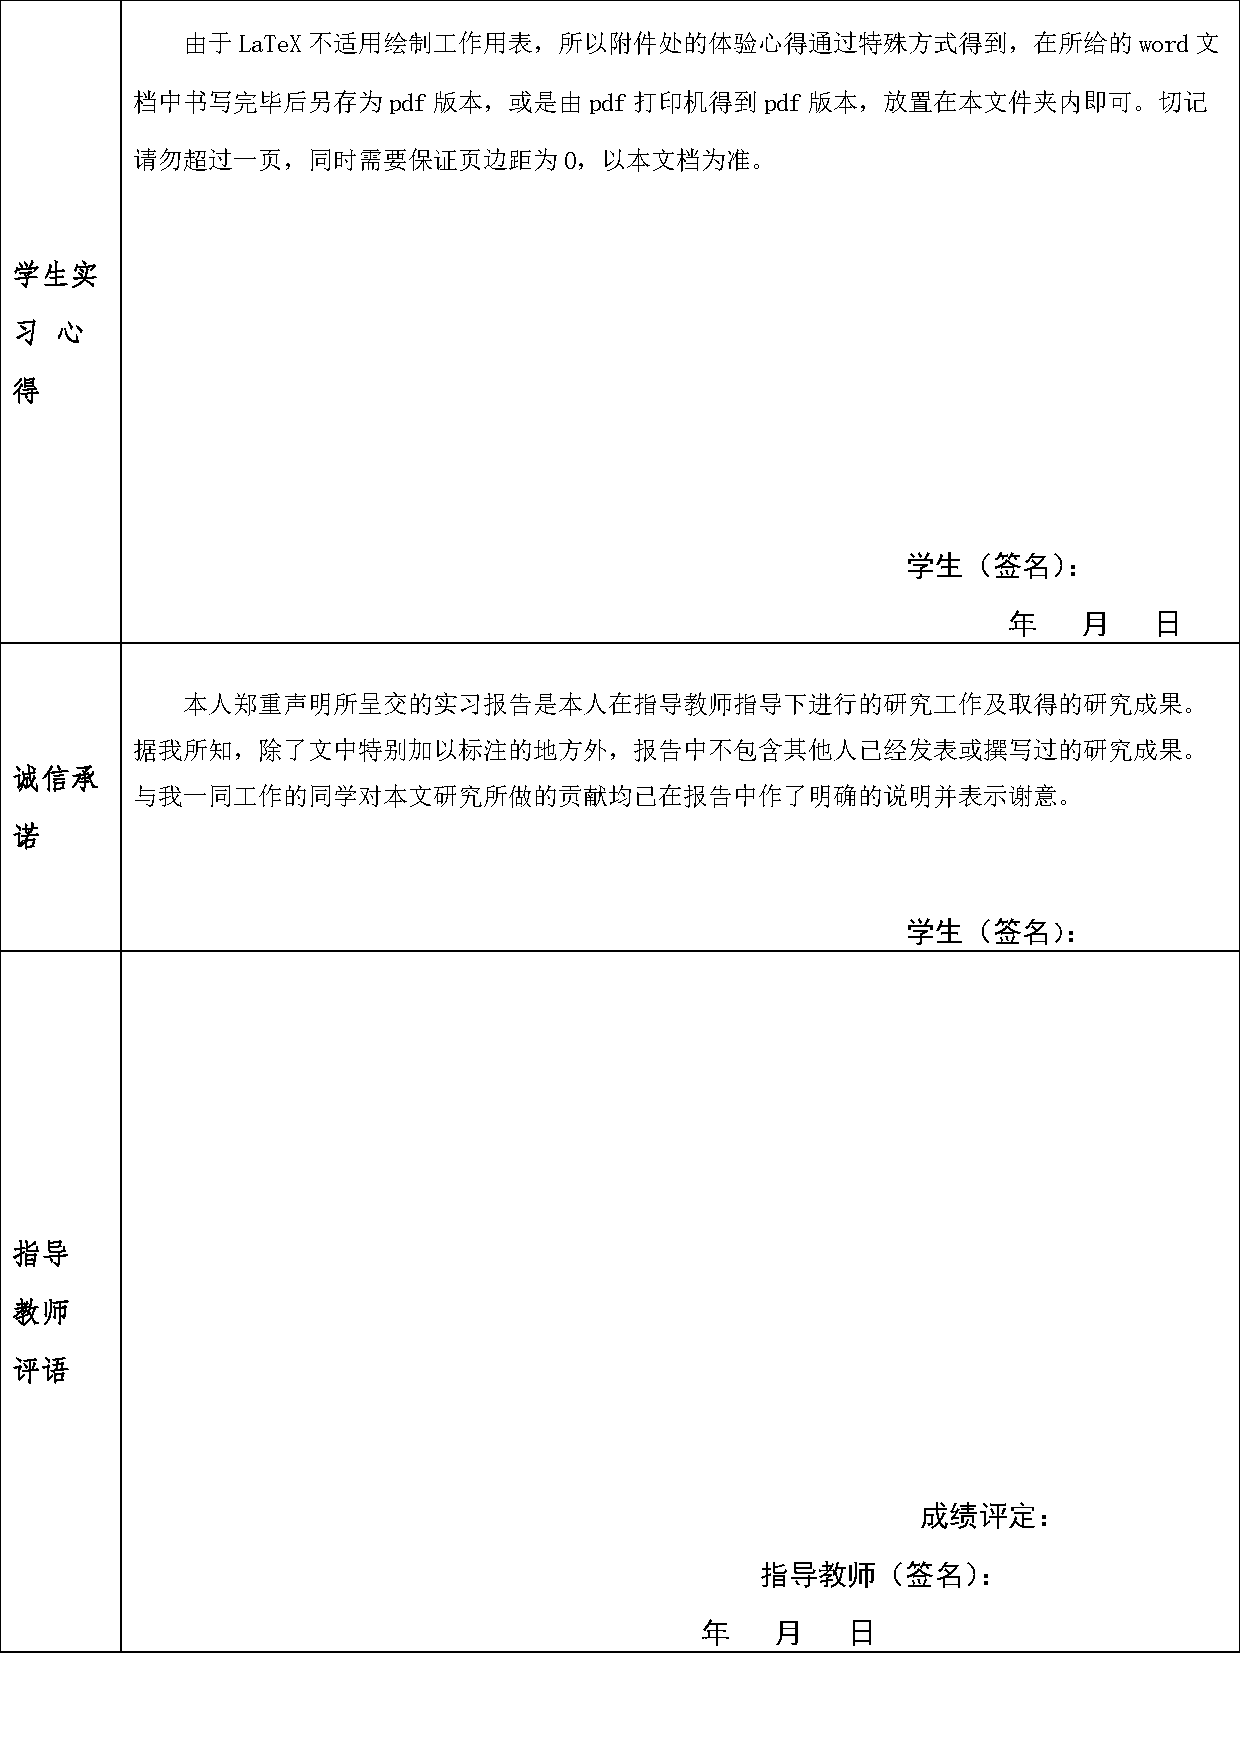
\includegraphics[width=15cm]{attachment/attachment.pdf}
\end{document}
\end{minted}

\verb|\doucumentclass[...]\{...}|称为设置文档类型,本模板使用成都理工大学的cdutlabreport类型。

在\verb|\doucumentclass|与\verb|\begin{document}|中间称为\textbf{导言区},学生需要在这里依次填写实验课程、实验名称、专业名称、学生姓名、学生学号、指导教师、实验地点和实验成绩,代替中括号内的内容即可。

文档内容使用\verb|\include{file}|逐个添加,便于整体管理的同时也使主文档美观简介。cover为文档封面与目录,\textbf{除特殊情况请勿更改},body内为文档各章节,attachment为学生实验心得。

文档实验报告内容从\verb|\begin{document}|开始,结束于\verb|\end{document}|。

由$\% !TeX$开头的两行为texstudio编辑器特有的魔法注释,意为使用UTF-8编码,编译引擎使用xelatex,由于本文代码高亮采用\verb|minted|包,所以添加了\verb|-shell-escape|,\textbf{若读者电脑中没有python环境,则无法正常编辑本文档,但不影响使用}。
\section{利用\LaTeX 排版中文文字}
\LaTeX 的源文件本质上是文本文档,利用Windows自带文本编辑器、note++、word、vim等文本编辑器均可编写出tex文档,至于texwork、texstudio、winedt等则为转述的tex编辑器,提供了语法高亮、匹配查找、自动补全命令等等用途。

除此之外\LaTeX 还可以排版数学公式、图片、表格等等,内容将在后续章节件数。
\subsection{\LaTeX 基本的命令与代码结构}
\LaTeX 命令均由反斜线$\backslash$开头,并为下列两种形式填空后续:
\begin{itemize}
\item 由反斜线$\backslash$与一连串字母组成,如\verb|\LaTeX|。注意在命令后需加空格或其他非字母作分隔符;
\item 由反斜线$\backslash$由后面的非字母符号组成,不需要分隔符,如\verb|\%|(百分号在\LaTeX 中为注释),为转义意。
\end{itemize}

注意\LaTeX 命令对\textbf{大小写是十分敏感的},比如输入\verb|\LaTeX|可以得到错落有致的\LaTeX 而输入\verb|\LaTex|或者\verb|\latex|则会报错,不会得到任何内容。

在\LaTeX 中的参数大多在$\{\cdots\}$或是在$[\cdots]$内,如之前所述\verb|\documentclass|\texttt{[CJK, GBK, UTF-8, oneside, a4paper, 12pt]{ctexart}}。
一些命令会在后面附带*号,带*号与不带*号结果不同。

为使一些状态、效果在局部生效,\LaTeX 引入了\textbf{环境}的用法,需要局部生效的内容被输入在环境内,由\verb|\begin{environment name}{arguments}|开始,由\verb|\end{environment}|结束。其中$environment$为环境名称,\verb|\begin{environment}|与\verb|\end{environment}|内的环境名应该一致,$arguments$为可选参数,环境之间允许嵌套使用。
\subsection{\LaTeX 排版中文}
排版中文文章时,与word不同,无需关注缩进、标题等等,在\LaTeX 中可以方便快捷的设置。一级标题设置代码为\verb|\section{title}|大括号内为一级标题的名称,对应的可以书写二级、三级标题,\LaTeX 命令分别为\verb|\subsection{title}|与\verb|\subsubsection{title}|。书写时,\LaTeX 会自动忽略文字中间的空格,在换行时需要多空一行。另外的,\LaTeX 中的注释为“\%”号。下面给出一个简短的例子。
\begin{minted}{LaTeX}
\section{一级标题名称}
这里是第一章的内容
% 空一行代表分段,百分号在LaTeX中代表注释
这里是第一章的内容
\subsection{二级标题名称}
这里是1.1的内容
\end{minted}

用户可以将代码放置在本模板中进行尝试,需要注意的是,在body文件夹内新建文档并书写完后,需要在主文档中依照给定格式导入新书写的文档。

在\LaTeX 中书写中文,无需注意文章标题的编号,在\verb|\section{title}|类命令中,自带有计数器,可以为标题自动编号,这使得用户无需关注排版格式,更多的关注在文档内容上。
\subsection{常用环境}
\subsubsection{居中}
在\LaTeX 中有两种居中方式:
\begin{itemize}
\item \verb|\centering|,在环境内使用,该环境内所有内容居中
\item \verb|center| 环境,在环境内的所有内容居中
\end{itemize}
\begin{center}
当使用了\verb|center|环境时候,环境内的所有内容都会被居中显示,且不会首行缩进。如果有特殊需要还可以使用flushleft 和flushright 环境,用于居左或者居右。
\end{center}
\subsubsection{带有编号的显示方式-列表(悬挂缩进)}
在书写实验报告时,经常会遇到需要分条叙述的方式,在一般书写排版中需要整体悬挂缩进。

在\LaTeX 中常用的两种环境,分别是itemize(无序)环境与enumerate环境(有序)两种环境可以互相嵌套使用,使用方法如下:
\begin{minted}{LaTeX}
% itemize环境
\begin{itemize}
\item 第一条内容
\item 第二条内容
\end{itemize}
% enumerate环境
\begin{enumerate}[aa.]
\item 第一条内容
\item 第二条内容
\end{enumerate}
\end{minted}
itemize环境会给每一条内容前加$\bullet$,而enumerate环境可以自定义,如(1. 2. 3.或者是A. B. C.),对应的设置方法需要在环境后的参数中写\verb|1.|、\verb|A.|,需要注意的是在给enumerate环境添加参数时候需要导入enumerate包,否则只会有\verb|1. 2. 3.|的序号,并且无法设置样式。
\begin{itemize}
\item 第一条内容
\item 第二条内容
\end{itemize}
\begin{enumerate}[a.]
\item 第一条内容第一条内容第一条内容第一条内容第一条内容第一条内容第一条内容第一条内容第一条内容第一条内容第一条内容第一条内容第一条内容第一条内容第一条内容第一条内容
\item 第二条内容
\end{enumerate}
\subsubsection{代码}
在实验报告中,多半部分需要加入对应的程序,编写代码的常用环境有verbatim、minted(需要python环境支持)、listings,下面分别叙述。

verbatim环境使用方法简单,但是不够美观,不能实现语法高亮。
\begin{verbatim}
#include<stdio.h>
int main(){
	printf("hello world");
	return 0;
}
\end{verbatim}

lstlisting环境需要listings包,可以自定义设置,本模板自带listings包并且给出了一种代码环境格式供用户参考。
\begin{lstlisting}{c}
#include<stdio.h>
int main(){
	printf("hello world");
	return 0;
}
\end{lstlisting}

minted环境需要minted包,并且电脑中安装有python环境。设置xelatex编译为\verb|xelatex.exe -synctex=1 -shell-escape -interaction=nonstopmode %.tex|,添加了\verb|-shell-escape|参数,可以胜任大部分计算机语言(Lingo除外),并且自动设置语法高亮。需要注意的是minted会将\verb|Tab|替换为下文中的\verb|^^I|,将所有的\verb|Tab|替换为空格即可,更多内容详见minted宏包文档,Win+R键后输入\verb|texdoc minted|即可查看minted宏包文档,在\LaTeX 中所有宏包的宏包文档均以上述方式打开。
\begin{minted}{C}
#include<stdio.h>
int main(){
	printf("hello world");
    return 0; /*将Tab替换为空格*/
}
\end{minted}

要排版简短的代码或关键字,可使用\verb|\verb| 命令:\verb|\verb<delim>\LaTeX<delim>|。
在该命令中所有的\verb|\|都不起作用。
\section{利用\LaTeX 排版数学公式}
在\LaTeX 中排版数学公式需要$amsmath$宏包(已经包含在本模板中),对多行公式的排版提供了有力的支持。在实验报告的书写中,主要以$amsmath$宏包的内容为主,其余内容不做阐述。
\subsection{公式排版基础}
在\LaTeX 中书写数学公式时必须带有数学环境,数学环境内可以识别特殊的命令并且字体改变为数学字体,一般数学环境有两种,书写方式如下:
\begin{itemize}
\item \textbf{行内公式:} 行内公式是出现在文字陈述中间的数学公式,需要用双\$符号括起来,例如我们知道对于矩阵而言,乘法交换率是不成立的,也就是说$\forall A\neq B,\, \exists A\times B\neq B\times      A$(\verb|$A\times B\neq B\times      A$|),书写时除去命令后必须的空格外,其他的空格会被一概忽略,至于如何添加空白会在后面叙述。
\item \textbf{行间公式:} 行间公式是出现在文字陈述段落中间的数学公式,一般需要编号。当行间公式需要编号时可以使用equation环境,不需要编号时可以使用简单的方式编写行间公式:\verb|\[myEquation\]|
\end{itemize}

在数学环境内,不允许有多于的空格与空行,需要强制空格可以使用命令\verb|\,|、\verb|\quad|、\verb|\qquad|等,他们的产生的空白距离有所不同。其次数学环境中的所有字母都会被当做变量处理,采用数学字体显示,当需要在数学环境中输入公式时,可以使用命令\verb|\text{}|。
\subsection{排版数学公式}
在以往的实验报告中,数学公式都会使用word中的mathtype书写,在较高的版本中可以复制mathtype为\LaTeX 代码,但这种投机取巧的方法写出来的符号会非常的丑,并且速度不会比直接使用\LaTeX 书写快多少。下面,作者会首先叙述一部分必要的知识,其次的内容会以实例的方式展现,需与tex文档(源文档)配合学习。

\begin{enumerate}[1.]
\item 上标的表示方式为\verb|a^{2}|,显示结果为$a^{2}$,当上标内容单一时可以省略大括号,如\verb|a^2|也可以显示为$a^2$,当需要输入符号$\^$时输入\verb|\^|即可。
\item 下表的表示方式为\verb|a_{2}|,显示结果为$a_{2}$,当小标内容单一时也可以省略大括号,当需要输入符号$\_$时输入\verb|\_|即可。
\item 同时需要上下标时书写没有先后顺序,\verb|a^{x+y}_{x_1}|与\verb|a_{x_1}^{x+y}|结果都是$a_{x_1}^{x+y}$。
\item 对于巨运算符,如果直接书写\verb|\sum^{n}_{i=1}n!|会容易显示为$\sum^{n}_{i=1}n!$,而添加命令\verb|\limits|后,\verb|\sum\limits^{n}_{i=1}n!|则会显示为$\sum\limits^{n}_{i=1}n!$。
\item 书写分数的命令为\verb|\frac{text}{den}|,其中text为分子部分,den部分为分母部分,如\verb|\frac{1}{2}|会显示为$\frac{1}{2}$,如果觉得分数略小可以适当的使用命令\verb|\dfrac{text}{den}|
显示为$\dfrac{1}{2}$。
\item 导数直接使用单引号即可\verb|f' f'' f'''|显示为$f' f'' f'''$,常见的运算符号与巨运算符如\verb|+ - \times \div = \sum \prod \int|,分别为$+ - \times \div = \sum \prod \int$,更多的基础符号见amsmath宏包或lshort,下面也给出了支持所有的符号大全与手写符号识别的网址。
\LaTeX 支持的符号大全:
\url{http://mirrors.ctan.org/info/symbols/comprehensive/symbols-a4.pdf}

手写符号识别:
\url{http://detexify.kirelabs.org/classify.html}
\item 需要输入大括号时需输入\verb|\{\}|。
\end{enumerate}
下面会用一些函数、习题、定理、证明过程或是计算过程作为实例:

\textbf{Stolz 定理}:设$\{y_n\}$是严格单调增加的正无穷大量,且
\[
\lim\limits_{n \to \infty}\frac{x_n-x_{n-1}}{y_n-y_{n-1}}=a\quad (a\text{可以为有限量,}+\infty\text{与}-\infty)\text{,}
\]
则
\[
\lim\limits_{n \to \infty}\frac{x_n}{y_n}=a\text{。}
\]

求极限
\[
\lim\limits_{n \to \infty}\frac{1^k+2^k+\cdots+n^k}{n^{k+1}}(k\text{为正整数})\text{。}
\]

由已知,可得
\begin{equation}\label{equ1}
\lim\limits_{n \to \infty}\frac{a^n}{n!}=0\text{。}
\end{equation}

设函数
\[
f(x)=(\frac{x+\exp^{\frac{1}{x}}}{1+\exp^{\frac{4}{x}}}+\frac{\sin x}{|x|})\text{,}
\]
问当$x\to 0$时,$f(x)$的极限是否存在?

设$f(x)$在$[a,b]$上连续,且$f(x)>0$,证明
\begin{equation}
\frac{1}{b-a}\int_{a}^{b}\ln f(x)\text{d}x\leqslant \ln \left(\frac{1}{b-a}\int_{a}^{b}f(x)\text{d}x\right)\text{。}
\end{equation}

常用的希腊字符如下:
\[\alpha \beta \gamma \delta \varepsilon \zeta \theta \eta \mu \xi \pi \sigma \omega \phi\]
\subsection{多行公式的排版}
在书写报告时,时长会遇到多行排版,如矩阵、分段函数等等,在下文将介绍部分常用的环境,用于排版多行公式。

多行排版的环境使用方式大致类似,需要对齐的位置利用$\&$分割,行末需要使用\verb|\\|分割。
\subsubsection{align环境}
align环境会给环境内的每一行公式编号,去掉编号可以使用\verb|\notag|,使用方式如下:
\begin{minted}{LaTeX}
\begin{align}
a & = b + c \\
a & = b + c \\
x + y & = d + e \notag
\end{align}
\end{minted}
显示为
\begin{align}
a & = b + c \\
a & = b + c \\
x + y & = d + e \notag
\end{align}

align环境会在$\&$符号处对齐,多个$\&$会分段对齐。
\subsubsection{aligned环境}
与align环境不同,aligned环境会给公式整体一个编号,而不是每一行都有编号,同时需要equation环境套在外面。
\begin{minted}{LaTeX}
\begin{equation}
	\begin{aligned}
		a & = b + c \\
		x + y & = d + e 
	\end{aligned}
\end{equation}
\end{minted}
显示为
\begin{equation}
	\begin{aligned}
		a & = b + c \\
		x + y & = d + e 
	\end{aligned}
\end{equation}
split 环境和aligned 环境用法类似,也用于和equation 环境套用,区别是split 只能
将每行的一个公式分两栏,aligned 允许每行多个公式多栏。
\subsubsection{array环境}
array环境用于排版数学数组、矩阵等,数组可作为一个公式块,在外套用\verb|\left|、\verb|\right|等定界符。跟在环境名后的\verb|{cccc}|意为矩阵4列均居中(c代表居中、l代表左对齐、r代表右对齐,更仔细的将在表格排版处讲述),具体实例如下:
\begin{minted}{LaTeX}
\[ 
\mathbf{X} = \left(
\begin{array}{cccc}
x_{11} & x_{12} & \ldots & x_{1n}\\
x_{21} & x_{22} & \ldots & x_{2n}\\
\vdots & \vdots & \ddots & \vdots\\
x_{n1} & x_{n2} & \ldots & x_{nn}\\
\end{array} \right) 
\]
\end{minted}
显示为
\[ 
\mathbf{X} = \left(
\begin{array}{cccc}
x_{11} & x_{12} & \ldots & x_{1n}\\
x_{21} & x_{22} & \ldots & x_{2n}\\
\vdots & \vdots & \ddots & \vdots\\
x_{n1} & x_{n2} & \ldots & x_{nn}\\
\end{array} \right) 
\]
其中,\verb|\left(|、\verb|\right)|就是矩阵的定界符,小括号可以替换为\verb|[ {|等。
\subsubsection{case环境}
借用之前所述的定界符,使用单侧定界符可以用来书写分段函数,如$\textbf{Riemann}$函数可以书写为:
\begin{minted}{LaTeX}
\[
\mathbf{R}(x)=\left\{\begin{array}{ll}
\frac{1}{p},&x=\frac{q}{p}(p\in \mathbf{N}^{+},q\in \mathbf{Z}-\{0\},p,q\text{互质}),\\
1,&x=0,\\
0,&x\text{为无理数}
\end{array}\right.
\]
\end{minted}
显示为
\[
\mathbf{R}(x)=\left\{\begin{array}{ll}
\frac{1}{p},&x=\frac{q}{p}(p\in \mathbf{N}^{+},q\in \mathbf{Z}-\{0\},p,q\text{互质}),\\
1,&x=0,\\
0,&x\text{为无理数}
\end{array}\right.
\]
对于这类分段函数,可以使用更简单的cases环境来完成
\begin{minted}{LaTeX}
\[
\mathbf{R}(x)=\begin{cases}
\frac{1}{p},&x=\frac{q}{p}(p\in \mathbf{N}^{+},q\in \mathbf{Z}-\{0\},p,q\text{互质}),\\
1,&x=0,\\
0,&x\text{为无理数}
\end{cases}
\]
\end{minted}
显示为
\[
\mathbf{R}(x)=\begin{cases}
\frac{1}{p},&x=\frac{q}{p}(p\in \mathbf{N}^{+},q\in \mathbf{Z}-\{0\},p,q\text{互质}),\\
1,&x=0,\\
0,&x\text{为无理数}
\end{cases}
\]
\section{利用\LaTeX 排版图片与表格}
在介绍如何排版表格与图片时,先介绍浮动体的概念
\subsection{浮动体}
在排版中文文档或者实验报告时,尤其是在今后的论文、书籍撰写中,表格与图片均称为\textbf{浮动体}。顾名思义,浮动体在文中的位置不是固定的,美观起见需要自动放在合适的位置,在需要的时候做引用。在排版时,作者需要优先排版文字内容,最后再关注图片位置,不应固定死图片的位置,除了造成大片空白也会使得整体不够美观。
\subsubsection{浮动体的用法}
一般来说浮动体环境有两种,figure环境与table环境,分别用于浮动图片与表格,用法如下:
\begin{minted}{LaTeX}
\begin{figure}[<placement>]
content...
\end{figure}
\end{minted}

表格与图片用法相同,跟在环境名后面的$placement$提供了浮动体在页面中允许排版的位置,默认为tbp,意为允许在顶部、底部、单独成页排版。
\begin{table}[h!]
\centering
\begin{tabular}{cc}
\hline
h&代码所处的当前位置\\
t&页面顶端\\
b&页码底部\\
p&单独成页\\
!&在决定位置时忽略限制\\
\hline
\end{tabular}
\end{table}
\subsubsection{浮动体的标题}
在浮动体中,利用\verb|\caption{...}|添加标题,用法与\verb|\section{...}|类似,添加的标题会自动编号,figure会在内容前显示如“图 1”的样式,表格类似。

紧跟着\verb|\caption{...}|后面可以添加\verb|\label{key}|命令交叉引用,具体在后面章节叙述。
\subsection{图片的排版}
\LaTeX 本身不支持插图功能,需要由graphicx 宏包(本模板已添加)辅助支持。在本模板下,可以添加.jpg.pdf.eps.png.bmp格式的图片,

在调用了graphicx包后,可以使用命令\verb|\includegraphics[⟨options⟩]{⟨filename⟩}|插入图片,$filename$是图片的位置,本模板中需要将图片放在figure文件中,并使用相对路径调用,如\verb|figure/filename.png|。$options$是需要的参数,如设置图片宽为0.7$cm$需要在该位置书写\verb|[width=0.7cm]|,具体的参数见表下表。
\begin{table}[h]
\centering
\begin{tabular}{lc}
\hline
参数&含义\\
\hline
width=h&将图片缩放到宽度为h\\
hight=h&将图片缩放到高度为h\\
scale=h&将图片按照原尺寸缩放h倍\\
angle=h&令图片逆时针旋转h度\\
\hline
\end{tabular}
\label{table1}
\end{table}

\begin{minted}{LaTeX}
\begin{figure}[h]
\centering
\includegraphics[scale = 0.7]{example-image-A}
\caption{导入的图片}
\label{fig1}
\end{figure}
\end{minted}
\begin{figure}[h]
\centering
\includegraphics[scale = 0.7]{example-image-A}
\caption{导入的图片}
\label{fig1}
\end{figure}
需要排版并排子图推荐使用subfig宏包,具体使用请看宏包文档
\subsection{表格的排版}
在实验报告或者论文中,表格是比不可少的部分。下面给出一个简单的表格排版实例:
\begin{minted}{LaTeX}
\begin{table}
\centering
\caption{表格排版实例}
\label{tab1}
\begin{tabular}{|c|l|r|}
\hline
AAA&B&CCC\\
\hline
A&BBB&C\\
\hline
\end{tabular}
\end{table}
\end{minted}

显示为表$^{[\ref{tab1}]}$。
\begin{table}[h]
\centering
\caption{表格排版实例}
\label{tab1}
\begin{tabular}{|c|l|r|}
\hline
AAA&B&CCC\\
\hline
A&BBB&C\\
\hline
\end{tabular}
\end{table}
与多行公式类似,表格排版中的列由tabular环境后的参数决定,c、l、r分别代表居中、居左、居右对齐,必须与列数相同,参数之间的竖线代表是否在表格中绘制竖线。行之间需要添加横线需要命令\verb|\hline|,如果需要合并单元格或者其他操作,具体见lshort表格排版章节,这里只讲述简单的部分。三线表的绘制只需要将参数中的竖线去除即可。

对于初次使用者而言,表格排版是一个很大的难题,在excel中有一个类似的插件可以快捷的生成大致的表格,在打开excel加载项后,下载插件\verb|excel2latex|即可。在生成大致表格后进行细微的调整,可以快速的绘制出想要的表格。
\section{交叉引用与其他}
\subsection{交叉引用}
在上一章我们强调了表格与图片需要在页面中自动寻找合适的位置,而不是固定在某个位置,那么我们需要引用表格内容时就不能用“如下表”类似的话语,而需要用到交叉引用,也就是“如图1”类似的文字。

细心的读者可以发现在浮动体环境内作者均加有\verb|\label{key}|的语句,这是为了后文方便引用图片内容而写,每个图片、表格的$key$值必须唯一。
在做引用的时候需要用到命令\verb|\ref{label}|,$label$处填写唯一的$key$值,这样就可以做到交叉引用,更方便的是在pdf阅读时,可以通过单击索引小标来定位到该图片处,如这里引用之前的图片就可以写如图$^{[\ref{fig1}]}$。

除了浮动体可以做交叉引用,公式也是可以做交叉引用的,这里引用文章出现的第一个公式可以写如公式$^{[\ref{equ1}]}$。

需要注意的是,目录与交叉引用需要至少编译两次,也就是点两次编译按钮。

由于本科实验报告中不要求添加参考文献,这里不做多于的叙述,详细的在lshort中也有叙述。
\subsection{其他}
这里将会叙述一些其他的知识,有的是在作者平时写作中遇到的,有的是模板写作中的问题,本章节会即时更新。

按照学校模板要求,在封面字体需为仿宋GB2312 加粗,事实上,字体的加粗并不想word中强制加粗(会出现很多很多很多错误),而是用其他粗体的字体来代替,因此本文由于版权限制,使用黑体代替格式中要求的字体。

在使用matlab绘图时,可以在图例、坐标轴等地方利用\LaTeX 公式写出分式等符号,但是matlab中只允许一部分\LaTeX 代码,并不是全部的数学公式代码都可以用。

\LaTeX 有相当多的宏包用于不同的环境,神经网络、化学、生物等等学科的图都可以在宏包中找到。
%----------------------------------------attachment--------------------------
\newpage
\thispagestyle{empty}
    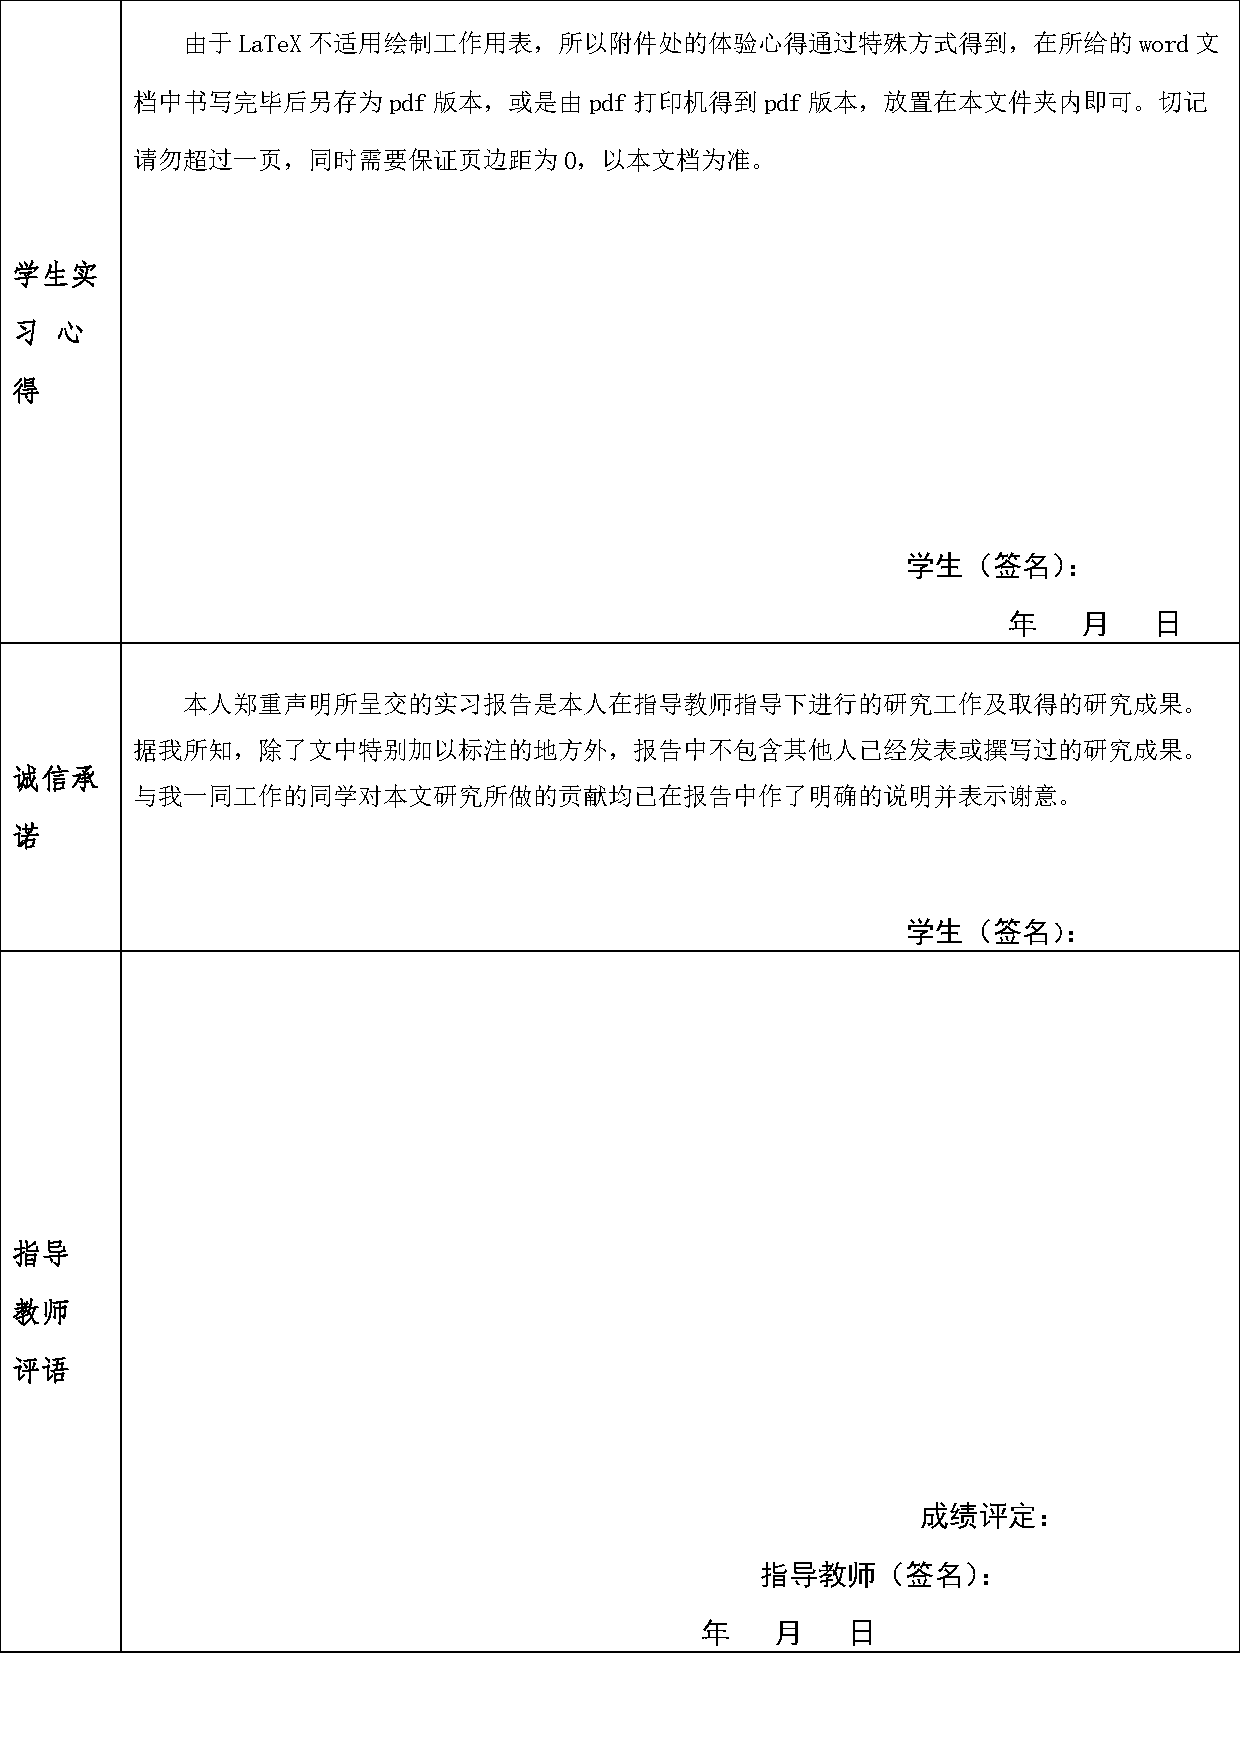
\includegraphics[width=15cm]{attachment/attachment.pdf}
\end{document}
\end{minted}

\verb|\doucumentclass[...]\{...}|称为设置文档类型,本模板使用成都理工大学的cdutlabreport类型。

在\verb|\doucumentclass|与\verb|\begin{document}|中间称为\textbf{导言区},学生需要在这里依次填写实验课程、实验名称、专业名称、学生姓名、学生学号、指导教师、实验地点和实验成绩,代替中括号内的内容即可。

文档内容使用\verb|\include{file}|逐个添加,便于整体管理的同时也使主文档美观简介。cover为文档封面与目录,\textbf{除特殊情况请勿更改},body内为文档各章节,attachment为学生实验心得。

文档实验报告内容从\verb|\begin{document}|开始,结束于\verb|\end{document}|。

由$\% !TeX$开头的两行为texstudio编辑器特有的魔法注释,意为使用UTF-8编码,编译引擎使用xelatex,由于本文代码高亮采用\verb|minted|包,所以添加了\verb|-shell-escape|,\textbf{若读者电脑中没有python环境,则无法正常编辑本文档,但不影响使用}。
\section{利用\LaTeX 排版中文文字}
\LaTeX 的源文件本质上是文本文档,利用Windows自带文本编辑器、note++、word、vim等文本编辑器均可编写出tex文档,至于texwork、texstudio、winedt等则为转述的tex编辑器,提供了语法高亮、匹配查找、自动补全命令等等用途。

除此之外\LaTeX 还可以排版数学公式、图片、表格等等,内容将在后续章节件数。
\subsection{\LaTeX 基本的命令与代码结构}
\LaTeX 命令均由反斜线$\backslash$开头,并为下列两种形式填空后续:
\begin{itemize}
\item 由反斜线$\backslash$与一连串字母组成,如\verb|\LaTeX|。注意在命令后需加空格或其他非字母作分隔符;
\item 由反斜线$\backslash$由后面的非字母符号组成,不需要分隔符,如\verb|\%|(百分号在\LaTeX 中为注释),为转义意。
\end{itemize}

注意\LaTeX 命令对\textbf{大小写是十分敏感的},比如输入\verb|\LaTeX|可以得到错落有致的\LaTeX 而输入\verb|\LaTex|或者\verb|\latex|则会报错,不会得到任何内容。

在\LaTeX 中的参数大多在$\{\cdots\}$或是在$[\cdots]$内,如之前所述\verb|\documentclass|\texttt{[CJK, GBK, UTF-8, oneside, a4paper, 12pt]{ctexart}}。
一些命令会在后面附带*号,带*号与不带*号结果不同。

为使一些状态、效果在局部生效,\LaTeX 引入了\textbf{环境}的用法,需要局部生效的内容被输入在环境内,由\verb|\begin{environment name}{arguments}|开始,由\verb|\end{environment}|结束。其中$environment$为环境名称,\verb|\begin{environment}|与\verb|\end{environment}|内的环境名应该一致,$arguments$为可选参数,环境之间允许嵌套使用。
\subsection{\LaTeX 排版中文}
排版中文文章时,与word不同,无需关注缩进、标题等等,在\LaTeX 中可以方便快捷的设置。一级标题设置代码为\verb|\section{title}|大括号内为一级标题的名称,对应的可以书写二级、三级标题,\LaTeX 命令分别为\verb|\subsection{title}|与\verb|\subsubsection{title}|。书写时,\LaTeX 会自动忽略文字中间的空格,在换行时需要多空一行。另外的,\LaTeX 中的注释为“\%”号。下面给出一个简短的例子。
\begin{minted}{LaTeX}
\section{一级标题名称}
这里是第一章的内容
% 空一行代表分段,百分号在LaTeX中代表注释
这里是第一章的内容
\subsection{二级标题名称}
这里是1.1的内容
\end{minted}

用户可以将代码放置在本模板中进行尝试,需要注意的是,在body文件夹内新建文档并书写完后,需要在主文档中依照给定格式导入新书写的文档。

在\LaTeX 中书写中文,无需注意文章标题的编号,在\verb|\section{title}|类命令中,自带有计数器,可以为标题自动编号,这使得用户无需关注排版格式,更多的关注在文档内容上。
\subsection{常用环境}
\subsubsection{居中}
在\LaTeX 中有两种居中方式:
\begin{itemize}
\item \verb|\centering|,在环境内使用,该环境内所有内容居中
\item \verb|center| 环境,在环境内的所有内容居中
\end{itemize}
\begin{center}
当使用了\verb|center|环境时候,环境内的所有内容都会被居中显示,且不会首行缩进。如果有特殊需要还可以使用flushleft 和flushright 环境,用于居左或者居右。
\end{center}
\subsubsection{带有编号的显示方式-列表(悬挂缩进)}
在书写实验报告时,经常会遇到需要分条叙述的方式,在一般书写排版中需要整体悬挂缩进。

在\LaTeX 中常用的两种环境,分别是itemize(无序)环境与enumerate环境(有序)两种环境可以互相嵌套使用,使用方法如下:
\begin{minted}{LaTeX}
% itemize环境
\begin{itemize}
\item 第一条内容
\item 第二条内容
\end{itemize}
% enumerate环境
\begin{enumerate}[aa.]
\item 第一条内容
\item 第二条内容
\end{enumerate}
\end{minted}
itemize环境会给每一条内容前加$\bullet$,而enumerate环境可以自定义,如(1. 2. 3.或者是A. B. C.),对应的设置方法需要在环境后的参数中写\verb|1.|、\verb|A.|,需要注意的是在给enumerate环境添加参数时候需要导入enumerate包,否则只会有\verb|1. 2. 3.|的序号,并且无法设置样式。
\begin{itemize}
\item 第一条内容
\item 第二条内容
\end{itemize}
\begin{enumerate}[a.]
\item 第一条内容第一条内容第一条内容第一条内容第一条内容第一条内容第一条内容第一条内容第一条内容第一条内容第一条内容第一条内容第一条内容第一条内容第一条内容第一条内容
\item 第二条内容
\end{enumerate}
\subsubsection{代码}
在实验报告中,多半部分需要加入对应的程序,编写代码的常用环境有verbatim、minted(需要python环境支持)、listings,下面分别叙述。

verbatim环境使用方法简单,但是不够美观,不能实现语法高亮。
\begin{verbatim}
#include<stdio.h>
int main(){
	printf("hello world");
	return 0;
}
\end{verbatim}

lstlisting环境需要listings包,可以自定义设置,本模板自带listings包并且给出了一种代码环境格式供用户参考。
\begin{lstlisting}{c}
#include<stdio.h>
int main(){
	printf("hello world");
	return 0;
}
\end{lstlisting}

minted环境需要minted包,并且电脑中安装有python环境。设置xelatex编译为\verb|xelatex.exe -synctex=1 -shell-escape -interaction=nonstopmode %.tex|,添加了\verb|-shell-escape|参数,可以胜任大部分计算机语言(Lingo除外),并且自动设置语法高亮。需要注意的是minted会将\verb|Tab|替换为下文中的\verb|^^I|,将所有的\verb|Tab|替换为空格即可,更多内容详见minted宏包文档,Win+R键后输入\verb|texdoc minted|即可查看minted宏包文档,在\LaTeX 中所有宏包的宏包文档均以上述方式打开。
\begin{minted}{C}
#include<stdio.h>
int main(){
	printf("hello world");
    return 0; /*将Tab替换为空格*/
}
\end{minted}

要排版简短的代码或关键字,可使用\verb|\verb| 命令:\verb|\verb<delim>\LaTeX<delim>|。
在该命令中所有的\verb|\|都不起作用。
\section{利用\LaTeX 排版数学公式}
在\LaTeX 中排版数学公式需要$amsmath$宏包(已经包含在本模板中),对多行公式的排版提供了有力的支持。在实验报告的书写中,主要以$amsmath$宏包的内容为主,其余内容不做阐述。
\subsection{公式排版基础}
在\LaTeX 中书写数学公式时必须带有数学环境,数学环境内可以识别特殊的命令并且字体改变为数学字体,一般数学环境有两种,书写方式如下:
\begin{itemize}
\item \textbf{行内公式:} 行内公式是出现在文字陈述中间的数学公式,需要用双\$符号括起来,例如我们知道对于矩阵而言,乘法交换率是不成立的,也就是说$\forall A\neq B,\, \exists A\times B\neq B\times      A$(\verb|$A\times B\neq B\times      A$|),书写时除去命令后必须的空格外,其他的空格会被一概忽略,至于如何添加空白会在后面叙述。
\item \textbf{行间公式:} 行间公式是出现在文字陈述段落中间的数学公式,一般需要编号。当行间公式需要编号时可以使用equation环境,不需要编号时可以使用简单的方式编写行间公式:\verb|\[myEquation\]|
\end{itemize}

在数学环境内,不允许有多于的空格与空行,需要强制空格可以使用命令\verb|\,|、\verb|\quad|、\verb|\qquad|等,他们的产生的空白距离有所不同。其次数学环境中的所有字母都会被当做变量处理,采用数学字体显示,当需要在数学环境中输入公式时,可以使用命令\verb|\text{}|。
\subsection{排版数学公式}
在以往的实验报告中,数学公式都会使用word中的mathtype书写,在较高的版本中可以复制mathtype为\LaTeX 代码,但这种投机取巧的方法写出来的符号会非常的丑,并且速度不会比直接使用\LaTeX 书写快多少。下面,作者会首先叙述一部分必要的知识,其次的内容会以实例的方式展现,需与tex文档(源文档)配合学习。

\begin{enumerate}[1.]
\item 上标的表示方式为\verb|a^{2}|,显示结果为$a^{2}$,当上标内容单一时可以省略大括号,如\verb|a^2|也可以显示为$a^2$,当需要输入符号$\^$时输入\verb|\^|即可。
\item 下表的表示方式为\verb|a_{2}|,显示结果为$a_{2}$,当小标内容单一时也可以省略大括号,当需要输入符号$\_$时输入\verb|\_|即可。
\item 同时需要上下标时书写没有先后顺序,\verb|a^{x+y}_{x_1}|与\verb|a_{x_1}^{x+y}|结果都是$a_{x_1}^{x+y}$。
\item 对于巨运算符,如果直接书写\verb|\sum^{n}_{i=1}n!|会容易显示为$\sum^{n}_{i=1}n!$,而添加命令\verb|\limits|后,\verb|\sum\limits^{n}_{i=1}n!|则会显示为$\sum\limits^{n}_{i=1}n!$。
\item 书写分数的命令为\verb|\frac{text}{den}|,其中text为分子部分,den部分为分母部分,如\verb|\frac{1}{2}|会显示为$\frac{1}{2}$,如果觉得分数略小可以适当的使用命令\verb|\dfrac{text}{den}|
显示为$\dfrac{1}{2}$。
\item 导数直接使用单引号即可\verb|f' f'' f'''|显示为$f' f'' f'''$,常见的运算符号与巨运算符如\verb|+ - \times \div = \sum \prod \int|,分别为$+ - \times \div = \sum \prod \int$,更多的基础符号见amsmath宏包或lshort,下面也给出了支持所有的符号大全与手写符号识别的网址。
\LaTeX 支持的符号大全:
\url{http://mirrors.ctan.org/info/symbols/comprehensive/symbols-a4.pdf}

手写符号识别:
\url{http://detexify.kirelabs.org/classify.html}
\item 需要输入大括号时需输入\verb|\{\}|。
\end{enumerate}
下面会用一些函数、习题、定理、证明过程或是计算过程作为实例:

\textbf{Stolz 定理}:设$\{y_n\}$是严格单调增加的正无穷大量,且
\[
\lim\limits_{n \to \infty}\frac{x_n-x_{n-1}}{y_n-y_{n-1}}=a\quad (a\text{可以为有限量,}+\infty\text{与}-\infty)\text{,}
\]
则
\[
\lim\limits_{n \to \infty}\frac{x_n}{y_n}=a\text{。}
\]

求极限
\[
\lim\limits_{n \to \infty}\frac{1^k+2^k+\cdots+n^k}{n^{k+1}}(k\text{为正整数})\text{。}
\]

由已知,可得
\begin{equation}\label{equ1}
\lim\limits_{n \to \infty}\frac{a^n}{n!}=0\text{。}
\end{equation}

设函数
\[
f(x)=(\frac{x+\exp^{\frac{1}{x}}}{1+\exp^{\frac{4}{x}}}+\frac{\sin x}{|x|})\text{,}
\]
问当$x\to 0$时,$f(x)$的极限是否存在?

设$f(x)$在$[a,b]$上连续,且$f(x)>0$,证明
\begin{equation}
\frac{1}{b-a}\int_{a}^{b}\ln f(x)\text{d}x\leqslant \ln \left(\frac{1}{b-a}\int_{a}^{b}f(x)\text{d}x\right)\text{。}
\end{equation}

常用的希腊字符如下:
\[\alpha \beta \gamma \delta \varepsilon \zeta \theta \eta \mu \xi \pi \sigma \omega \phi\]
\subsection{多行公式的排版}
在书写报告时,时长会遇到多行排版,如矩阵、分段函数等等,在下文将介绍部分常用的环境,用于排版多行公式。

多行排版的环境使用方式大致类似,需要对齐的位置利用$\&$分割,行末需要使用\verb|\\|分割。
\subsubsection{align环境}
align环境会给环境内的每一行公式编号,去掉编号可以使用\verb|\notag|,使用方式如下:
\begin{minted}{LaTeX}
\begin{align}
a & = b + c \\
a & = b + c \\
x + y & = d + e \notag
\end{align}
\end{minted}
显示为
\begin{align}
a & = b + c \\
a & = b + c \\
x + y & = d + e \notag
\end{align}

align环境会在$\&$符号处对齐,多个$\&$会分段对齐。
\subsubsection{aligned环境}
与align环境不同,aligned环境会给公式整体一个编号,而不是每一行都有编号,同时需要equation环境套在外面。
\begin{minted}{LaTeX}
\begin{equation}
	\begin{aligned}
		a & = b + c \\
		x + y & = d + e 
	\end{aligned}
\end{equation}
\end{minted}
显示为
\begin{equation}
	\begin{aligned}
		a & = b + c \\
		x + y & = d + e 
	\end{aligned}
\end{equation}
split 环境和aligned 环境用法类似,也用于和equation 环境套用,区别是split 只能
将每行的一个公式分两栏,aligned 允许每行多个公式多栏。
\subsubsection{array环境}
array环境用于排版数学数组、矩阵等,数组可作为一个公式块,在外套用\verb|\left|、\verb|\right|等定界符。跟在环境名后的\verb|{cccc}|意为矩阵4列均居中(c代表居中、l代表左对齐、r代表右对齐,更仔细的将在表格排版处讲述),具体实例如下:
\begin{minted}{LaTeX}
\[ 
\mathbf{X} = \left(
\begin{array}{cccc}
x_{11} & x_{12} & \ldots & x_{1n}\\
x_{21} & x_{22} & \ldots & x_{2n}\\
\vdots & \vdots & \ddots & \vdots\\
x_{n1} & x_{n2} & \ldots & x_{nn}\\
\end{array} \right) 
\]
\end{minted}
显示为
\[ 
\mathbf{X} = \left(
\begin{array}{cccc}
x_{11} & x_{12} & \ldots & x_{1n}\\
x_{21} & x_{22} & \ldots & x_{2n}\\
\vdots & \vdots & \ddots & \vdots\\
x_{n1} & x_{n2} & \ldots & x_{nn}\\
\end{array} \right) 
\]
其中,\verb|\left(|、\verb|\right)|就是矩阵的定界符,小括号可以替换为\verb|[ {|等。
\subsubsection{case环境}
借用之前所述的定界符,使用单侧定界符可以用来书写分段函数,如$\textbf{Riemann}$函数可以书写为:
\begin{minted}{LaTeX}
\[
\mathbf{R}(x)=\left\{\begin{array}{ll}
\frac{1}{p},&x=\frac{q}{p}(p\in \mathbf{N}^{+},q\in \mathbf{Z}-\{0\},p,q\text{互质}),\\
1,&x=0,\\
0,&x\text{为无理数}
\end{array}\right.
\]
\end{minted}
显示为
\[
\mathbf{R}(x)=\left\{\begin{array}{ll}
\frac{1}{p},&x=\frac{q}{p}(p\in \mathbf{N}^{+},q\in \mathbf{Z}-\{0\},p,q\text{互质}),\\
1,&x=0,\\
0,&x\text{为无理数}
\end{array}\right.
\]
对于这类分段函数,可以使用更简单的cases环境来完成
\begin{minted}{LaTeX}
\[
\mathbf{R}(x)=\begin{cases}
\frac{1}{p},&x=\frac{q}{p}(p\in \mathbf{N}^{+},q\in \mathbf{Z}-\{0\},p,q\text{互质}),\\
1,&x=0,\\
0,&x\text{为无理数}
\end{cases}
\]
\end{minted}
显示为
\[
\mathbf{R}(x)=\begin{cases}
\frac{1}{p},&x=\frac{q}{p}(p\in \mathbf{N}^{+},q\in \mathbf{Z}-\{0\},p,q\text{互质}),\\
1,&x=0,\\
0,&x\text{为无理数}
\end{cases}
\]
\section{利用\LaTeX 排版图片与表格}
在介绍如何排版表格与图片时,先介绍浮动体的概念
\subsection{浮动体}
在排版中文文档或者实验报告时,尤其是在今后的论文、书籍撰写中,表格与图片均称为\textbf{浮动体}。顾名思义,浮动体在文中的位置不是固定的,美观起见需要自动放在合适的位置,在需要的时候做引用。在排版时,作者需要优先排版文字内容,最后再关注图片位置,不应固定死图片的位置,除了造成大片空白也会使得整体不够美观。
\subsubsection{浮动体的用法}
一般来说浮动体环境有两种,figure环境与table环境,分别用于浮动图片与表格,用法如下:
\begin{minted}{LaTeX}
\begin{figure}[<placement>]
content...
\end{figure}
\end{minted}

表格与图片用法相同,跟在环境名后面的$placement$提供了浮动体在页面中允许排版的位置,默认为tbp,意为允许在顶部、底部、单独成页排版。
\begin{table}[h!]
\centering
\begin{tabular}{cc}
\hline
h&代码所处的当前位置\\
t&页面顶端\\
b&页码底部\\
p&单独成页\\
!&在决定位置时忽略限制\\
\hline
\end{tabular}
\end{table}
\subsubsection{浮动体的标题}
在浮动体中,利用\verb|\caption{...}|添加标题,用法与\verb|\section{...}|类似,添加的标题会自动编号,figure会在内容前显示如“图 1”的样式,表格类似。

紧跟着\verb|\caption{...}|后面可以添加\verb|\label{key}|命令交叉引用,具体在后面章节叙述。
\subsection{图片的排版}
\LaTeX 本身不支持插图功能,需要由graphicx 宏包(本模板已添加)辅助支持。在本模板下,可以添加.jpg.pdf.eps.png.bmp格式的图片,

在调用了graphicx包后,可以使用命令\verb|\includegraphics[⟨options⟩]{⟨filename⟩}|插入图片,$filename$是图片的位置,本模板中需要将图片放在figure文件中,并使用相对路径调用,如\verb|figure/filename.png|。$options$是需要的参数,如设置图片宽为0.7$cm$需要在该位置书写\verb|[width=0.7cm]|,具体的参数见表下表。
\begin{table}[h]
\centering
\begin{tabular}{lc}
\hline
参数&含义\\
\hline
width=h&将图片缩放到宽度为h\\
hight=h&将图片缩放到高度为h\\
scale=h&将图片按照原尺寸缩放h倍\\
angle=h&令图片逆时针旋转h度\\
\hline
\end{tabular}
\label{table1}
\end{table}

\begin{minted}{LaTeX}
\begin{figure}[h]
\centering
\includegraphics[scale = 0.7]{example-image-A}
\caption{导入的图片}
\label{fig1}
\end{figure}
\end{minted}
\begin{figure}[h]
\centering
\includegraphics[scale = 0.7]{example-image-A}
\caption{导入的图片}
\label{fig1}
\end{figure}
需要排版并排子图推荐使用subfig宏包,具体使用请看宏包文档
\subsection{表格的排版}
在实验报告或者论文中,表格是比不可少的部分。下面给出一个简单的表格排版实例:
\begin{minted}{LaTeX}
\begin{table}
\centering
\caption{表格排版实例}
\label{tab1}
\begin{tabular}{|c|l|r|}
\hline
AAA&B&CCC\\
\hline
A&BBB&C\\
\hline
\end{tabular}
\end{table}
\end{minted}

显示为表$^{[\ref{tab1}]}$。
\begin{table}[h]
\centering
\caption{表格排版实例}
\label{tab1}
\begin{tabular}{|c|l|r|}
\hline
AAA&B&CCC\\
\hline
A&BBB&C\\
\hline
\end{tabular}
\end{table}
与多行公式类似,表格排版中的列由tabular环境后的参数决定,c、l、r分别代表居中、居左、居右对齐,必须与列数相同,参数之间的竖线代表是否在表格中绘制竖线。行之间需要添加横线需要命令\verb|\hline|,如果需要合并单元格或者其他操作,具体见lshort表格排版章节,这里只讲述简单的部分。三线表的绘制只需要将参数中的竖线去除即可。

对于初次使用者而言,表格排版是一个很大的难题,在excel中有一个类似的插件可以快捷的生成大致的表格,在打开excel加载项后,下载插件\verb|excel2latex|即可。在生成大致表格后进行细微的调整,可以快速的绘制出想要的表格。
\section{交叉引用与其他}
\subsection{交叉引用}
在上一章我们强调了表格与图片需要在页面中自动寻找合适的位置,而不是固定在某个位置,那么我们需要引用表格内容时就不能用“如下表”类似的话语,而需要用到交叉引用,也就是“如图1”类似的文字。

细心的读者可以发现在浮动体环境内作者均加有\verb|\label{key}|的语句,这是为了后文方便引用图片内容而写,每个图片、表格的$key$值必须唯一。
在做引用的时候需要用到命令\verb|\ref{label}|,$label$处填写唯一的$key$值,这样就可以做到交叉引用,更方便的是在pdf阅读时,可以通过单击索引小标来定位到该图片处,如这里引用之前的图片就可以写如图$^{[\ref{fig1}]}$。

除了浮动体可以做交叉引用,公式也是可以做交叉引用的,这里引用文章出现的第一个公式可以写如公式$^{[\ref{equ1}]}$。

需要注意的是,目录与交叉引用需要至少编译两次,也就是点两次编译按钮。

由于本科实验报告中不要求添加参考文献,这里不做多于的叙述,详细的在lshort中也有叙述。
\subsection{其他}
这里将会叙述一些其他的知识,有的是在作者平时写作中遇到的,有的是模板写作中的问题,本章节会即时更新。

按照学校模板要求,在封面字体需为仿宋GB2312 加粗,事实上,字体的加粗并不想word中强制加粗(会出现很多很多很多错误),而是用其他粗体的字体来代替,因此本文由于版权限制,使用黑体代替格式中要求的字体。

在使用matlab绘图时,可以在图例、坐标轴等地方利用\LaTeX 公式写出分式等符号,但是matlab中只允许一部分\LaTeX 代码,并不是全部的数学公式代码都可以用。

\LaTeX 有相当多的宏包用于不同的环境,神经网络、化学、生物等等学科的图都可以在宏包中找到。
%----------------------------------------attachment--------------------------
\newpage
\thispagestyle{empty}
    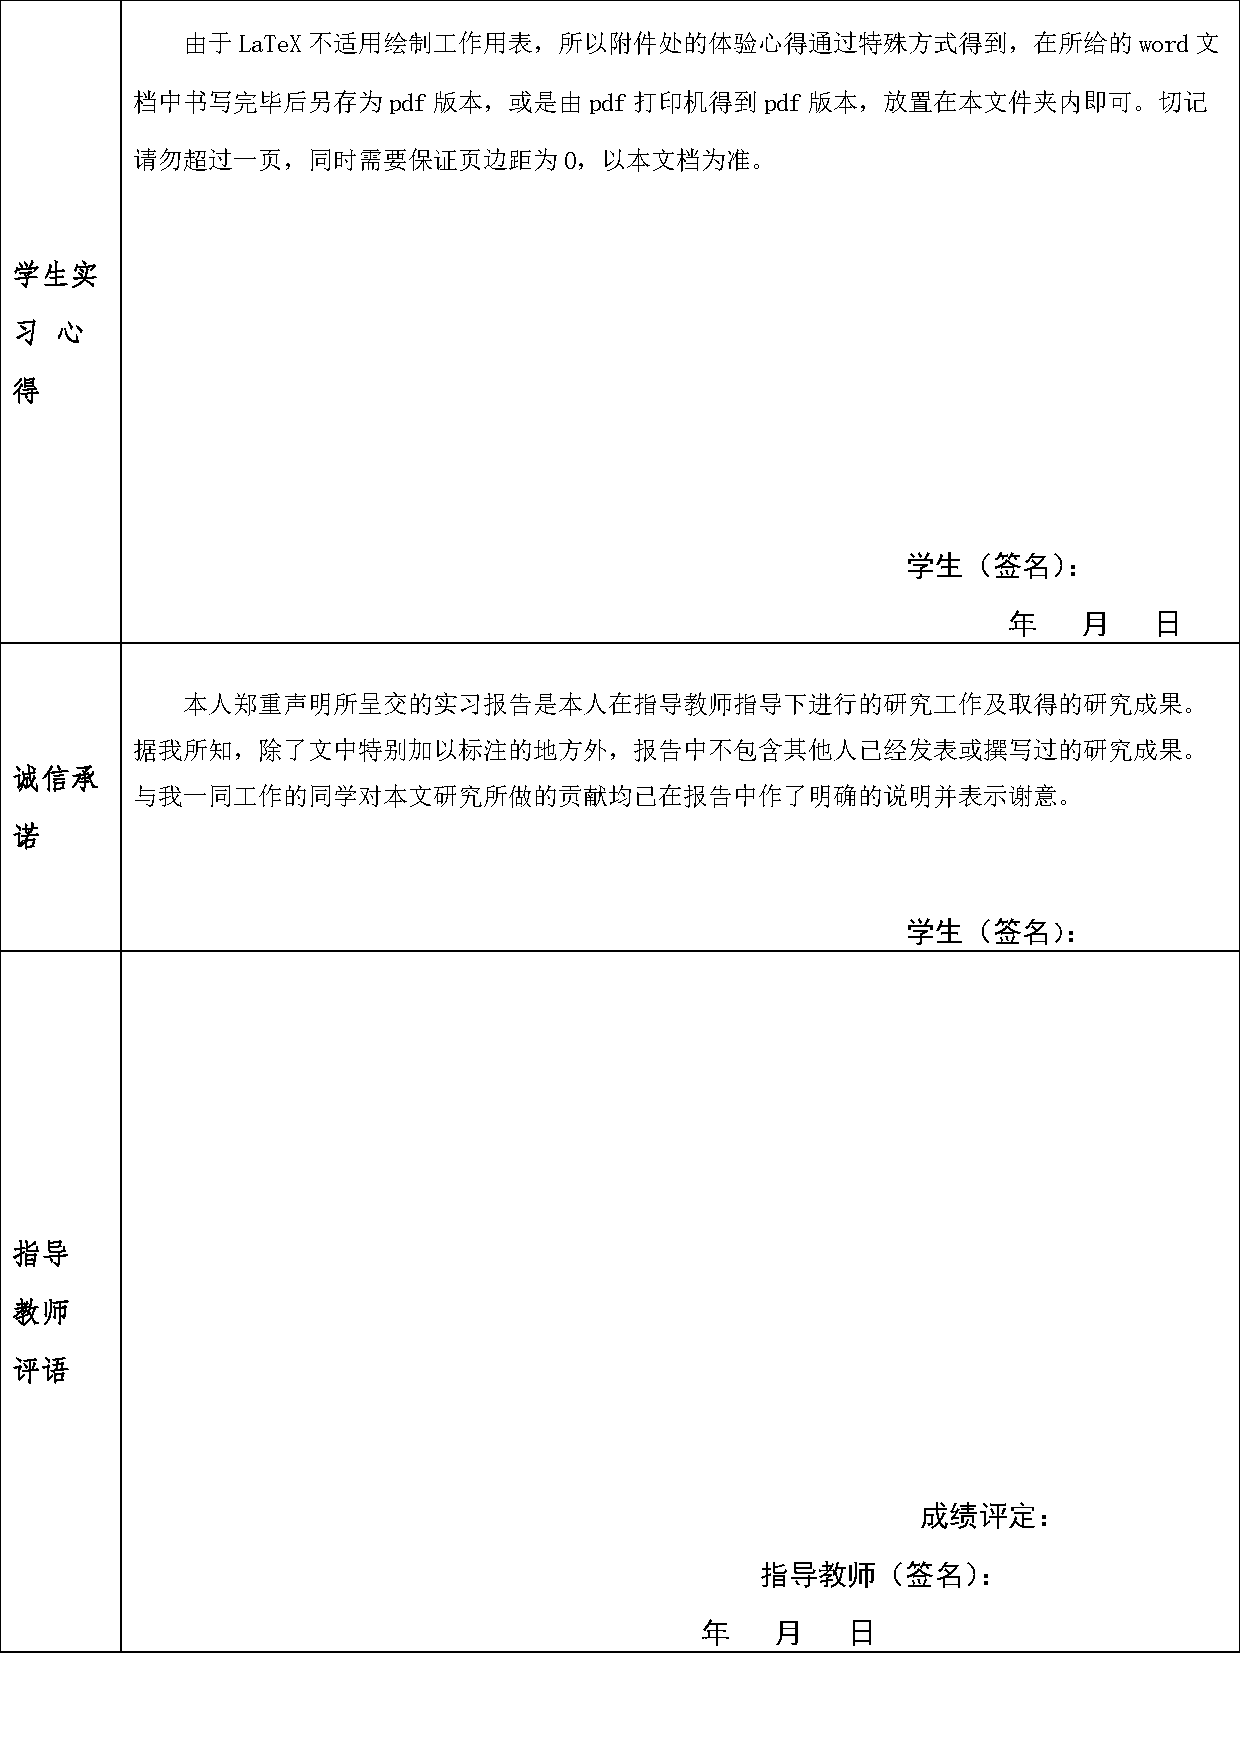
\includegraphics[width=15cm]{attachment/attachment.pdf}
\end{document}
\end{minted}

\verb|\doucumentclass[...]\{...}|称为设置文档类型,本模板使用成都理工大学的cdutlabreport类型。

在\verb|\doucumentclass|与\verb|\begin{document}|中间称为\textbf{导言区},学生需要在这里依次填写实验课程、实验名称、专业名称、学生姓名、学生学号、指导教师、实验地点和实验成绩,代替中括号内的内容即可。

文档内容使用\verb|\include{file}|逐个添加,便于整体管理的同时也使主文档美观简介。cover为文档封面与目录,\textbf{除特殊情况请勿更改},body内为文档各章节,attachment为学生实验心得。

文档实验报告内容从\verb|\begin{document}|开始,结束于\verb|\end{document}|。

由$\% !TeX$开头的两行为texstudio编辑器特有的魔法注释,意为使用UTF-8编码,编译引擎使用xelatex,由于本文代码高亮采用\verb|minted|包,所以添加了\verb|-shell-escape|,\textbf{若读者电脑中没有python环境,则无法正常编辑本文档,但不影响使用}。